% !TeX root = main.tex
%!TeX root = main.tex
\documentclass[nonacm,sigplan,natbib=false]{acmart}
\usepackage{amsmath}
\usepackage{enumitem}
\usepackage{algorithm}
\usepackage[noend]{algpseudocode}
\usepackage[datamodel=acmdatamodel,style=acmnumeric]{biblatex}
\usepackage{mathtools}
\usepackage{tikz}
\usepackage{booktabs}
\usepackage{subcaption}
\usepackage{varioref}
\usepackage{hyperref}
\usepackage{cleveref}

\pagestyle{plain}
\settopmatter{printfolios=true}

\usetikzlibrary{arrows.meta}
\usetikzlibrary{positioning}

\providecommand{\giv}{\:\vert\:}

\DeclareMathOperator*{\argmax}{arg\,max}
\DeclareMathOperator*{\argmin}{arg\,min}
\DeclarePairedDelimiter{\seq}{\langle}{\rangle}
\DeclarePairedDelimiterX{\pan}[1]{(}{)}{\renewcommand{\giv}{\:\delimsize\vert\:}#1}
\DeclarePairedDelimiter{\lis}{[}{]}
\DeclarePairedDelimiterX{\set}[1]{\{}{\}}{\renewcommand{\giv}{\:\delimsize\vert\:}#1}

\DeclareMathOperator{\prob}{\mathbb{P}}

\newlist{researchquestions}{enumerate}{1}
\setlist[researchquestions]{label*=\textbf{RQ~\arabic*}, ref=\arabic*}
\crefname{researchquestionsi}{RQ}{RQs}

\tikzset{
    box/.style={
        rectangle,
        draw,
        thick,
        rounded corners=4pt,
        fill=white,
    },
    arr/.tip={Latex[round]}
}

\newcommand{\worklogalpha}{$\textsc{WorkLog}_\alpha$}
\newcommand{\worklogbeta}{$\textsc{WorkLog}_\beta$}

\title{Project Final Report: Modeling and Generating Realistic Workloads}
\author{JianChen Zhao}
\email{jianchen.zhao@uwaterloo.ca}
\addbibresource{paperpile.bib}

\begin{document}

\begin{abstract}
    As software systems become more complex and deployed on increasingly diverse platforms, the need for load testing and quality workloads is also increased. Load testing is required to ensure the proper functioning of a software system under a realistic environment and can find potential issues that functional tests cannot find. In order for load testing to be effective, one needs to input a realistic workload. Collecting user inputs is costly and complex. Thus, many research works propose automatic workload reproduction approaches. However, many of those approaches do not consider noise and the ability to extrapolate novel action sequences. We propose to use an interleaved HMM to learn the user behavior through event logs, which are then used to generate action sequences. We describe in detail the formulation of the approach and techniques used. We implement two variants of our approach, \worklogalpha{} and \worklogbeta{}. We show through an extensive evaluation that our approach can generate realistic yet diverse workloads while also being customizable to the use case.
\end{abstract}

\maketitle

\section{Introduction}

In today's dynamic and interconnected digital landscape, where user expectations for speed and reliability are higher than ever, workload testing is indispensable. For instance, Ticketmaster, a well-known ticket vendor, faced technical difficulties such as server crashes and increased latency during a pre-sale event for Taylor Swift's 2022 tour. Despite preregistrations for the event, their system faltered due to inadequate load testing \cite{Reuters2022-dc}. This incident resulted in public backlash and multiple lawsuits. In contrast, during Prime Day 2023, Amazon handled an astounding number of requests, including 764 petabytes of EBS data transfer, over 15.35 trillion requests, 830 CloudTrail events, and 500 million CloudFront HTTP requests per minute. Amazon would not have achieved such a feat without rigorous load testing\cite{Barr2023-wr}.

As software systems become more complex and are deployed on increasingly diverse platforms, assessing their robustness under varying workloads becomes paramount. Large-scale software systems like cloud services are deeply embedded into today's economy. Many businesses's critical operations rely on such software. To illustrate, the global end-user spending in public cloud services is more than half a trillion USD in 2023\cite{UnknownUnknown-aj}. For operators of such large-scale software systems, a failure can result in significant financial loss and impact business worldwide\cite{LuuUnknown-mo}; Facebook, for example, lost an estimated 90 million USD to a 14-hour outage caused by misconfigured DNS\cite{AtlassianUnknown-sw}. Interestingly, such failures can not be attributed to functional bugs\cite{Weyuker2000-gw}. It is, therefore, crucial that systems are rigorously tested as a whole.

\subsection{Background}

Among the various system testing paradigms, load testing emerges as a critical aspect, focusing on the system's ability to handle different levels of expected user activity. This form of testing empirically guarantees that a software application can meet its performance objectives under realistic working conditions.

Load testing involves simulating different scenarios and conditions that mimic the actual usage patterns and demands the software may encounter in a production environment. Subjecting the system to \emph{workloads}, including typical and peak loads, reduces system failure risks while helping identify potential bottlenecks, vulnerabilities, or performance degradation that may not arise in functional tests \cite{Syer2017-ek, Shang2015-gj, Cohen2005-mn, Hassan2008-nj, Chen2016-bo}.

We define a workload as a sequence of actions to which we can subject a system under test. In research and practice, there are many ways one might obtain workloads.

The most basic form of load testing consists of replaying the system against a manually collected dataset of user actions. This approach requires extensive tooling of the deployed system to capture the user actions and ample storage to accommodate the large number of workloads necessary to capture the variance in user actions. Many prior works have explored the automatically recovering workloads to work around these issues.

However, automatically generating workloads is no trivial task. There are two main challenges. First, the generated workload must be realistic. The action patterns in the workload must be representative of actual field observations. This property is essential to the usefulness of load testing. Testing on unrealistic data cannot ensure that the system under test can handle actual user actions. Second, real user actions have high variance; that is, there is a diverse number of action patterns in production environments. Hence, automatic workload generation techniques must balance the variance and representativeness of the recovered workload.

\subsection{Related Work}

Prior works on workload generation have explored automatically recovering workloads from various readily available sources, which are resampled for replay.

Many proposed approaches abstract away user behaviors in workload and only consider specific metrics. This reduces the information needed to be stored for replay. \cite{Shang2015-gj, Cohen2005-mn} use CPU usage metrics for high-level representation of user behaviors. Similarly, \cite{Haghdoost2017-bc, Yadwadkar2010-ml, Busch2015-yo, Seo2014-xv} characterize the load by the I/O usage, while \cite{Cortez2017-nc} looks at other system resource usage to model the workloads. While such coarse-grained approaches are efficient and easy to maintain, information about essential characteristics of the load might be lost.

As demonstrated in \cite{Cohen2005-mn}, more precise characterization of workloads may lead to better performance. \cite{Yadwadkar2010-ml} explored using a hidden Markov model to find patterns of user behaviors and found that only a small amount of data is required to construct an adequate model of the user behaviors.

To balance the granularity of the recovered workloads, \cite{Syer2017-ek, Vogele2018-zz, Summers2016-jj, Xi2011-ki, Hassan2008-nj} distinguishes different user behaviors by clustering user actions extracted from event logs or system traces. \cite{Chen2019-fu} adds to this approach by also considering sequences of user actions and their context, helping find more representative user behaviors without sacrificing the variance of the recovered workloads and introducing some adaptability to the approach. While this approach can achieve a good balance, it suffers from two problems. First, the approach clusters users based on their behaviors to sample actions and action sequences of a recovered workload using representative users. In effect, the diversity of the generated workload is restricted by the size of the source used to recover the initial workload. Second, event logs and traces are noisy. Actions are thus recovered by filtering on some user identifiers. However, those identifiers are not always present, and the recovered actions may be incomplete \cite{Zhao2023-nh}. We extend \cite{Chen2019-fu} with ideas from \cite{Yadwadkar2010-ml} to achieve the ability to generate realistic yet novel and high-variance workloads.

\subsection{Contributions}

To tackle the challenges above, we propose an extensible model of user behaviors found in event logs based on a mixture of Hidden Markov Models (HMM) to allow the dynamic generation of workloads unconstrained by the size of the initial recovered workload. We evaluate our model and demonstrate its performance and generalizability. We also propose directions for future improvements.

\subsection{Organization}

We present our model in detail in \cref{sec:modeling_processes} while highlighting challenges in training such a model. We show in \cref{sec:approach} how it can be integrated to generate workloads dynamically. We evaluate it in \cref{sec:experimental_setup,sec:results}, and discuss tradeoffs and potential improvements in \cref{sec:discussion}. Finally, we conclude in \cref{sec:conclusion}.

\section{Modeling Event Logs}\label{sec:modeling_processes}

Event logs and system traces are discrete-time processes. Given time steps \(1, 2, ..., t, ..., \tau - 1, \tau\),  events \(y_t\) are observed according to an underlying process, that is, the control flow of a running software system.

\subsection{Control Flow Graph}

The control flow graph (CFG) of a program can be understood as the graphical representation of its state transitions at runtime. Nodes in this graph represent sequences of statements executed sequentially without branching except at the entry and exit statements. Edges represent the control flow and its branching between the basic blocks.

The CFG can also be seen as a description of the underlying process that produces outputs and, for our purposes, event logs and system traces. However, to get a complete picture of the production process, we need to compute the CFG for the whole program, or in other words, the interprocedural CFG (ICFG). Computing this ICFG is resource-intensive, impractical, and often outright impossible. It must thus be approximated\cite{Zhao2023-nh}.

\subsection{Hidden Markov Chains (HMM)}

\begin{figure}
    \caption{An example of a graph of the states of a process, with associated state transition probabilities. This graph is analogous to a control flow graph.}
    \label{fig:state_graph}
    \vspace{2ex}
    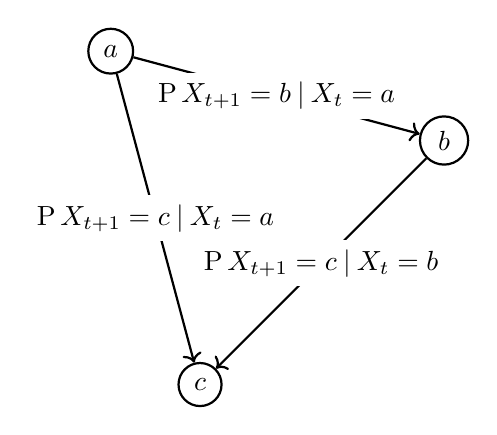
\begin{tikzpicture}[x=1pt,y=1pt]
        \node [box,circle] (a) at (135:72) {$a$};
        \node [box,circle] (b) at (015:72) {$b$};
        \node [box,circle] (c) at (255:72) {$c$};
        \draw [->,thick] (a) -- (b) node [midway,fill=white] {$\prob\pan{X_{t+1} = b \giv X_t = a}$};
        \draw [->,thick] (a) -- (c) node [midway,fill=white] {$\prob\pan{X_{t+1} = c \giv X_t = a}$};
        \draw [->,thick] (b) -- (c) node [midway,fill=white] {$\prob\pan{X_{t+1} = c \giv X_t = b}$};
    \end{tikzpicture}
\end{figure}

Instead of directly approximating an ICFG, we can fit a hidden Markov model (HMM) on a program's output to learn its states and transitions at runtime. In this approach, we do not require the use of source code. The learned graph, where nodes are states and edges are transitions, is an indirect approximation of the ICFG with respect to the output. That is, it models the process that generates the outputs.

A HMM \(\mu = (X, Y)\) consists of two stochastic processes: \(X = \{X_t : 0 \leq t \leq \tau\}\) is a Markov process that is not directly observable, hence hidden, and \(Y = \{Y_t : 0 \leq t \leq \tau\}\) that is directly observed. Each \(X_t\) only depends on the previous \(X_{t-1}\) and each \(Y_t\) only depends on \(X_t\).

For simplicity, we assume that \(X\) is ergodic; that is, the probability of getting from every state to every other state is non-zero. This assumption should hold in practice; for load testing, we are concerned with system states that are reoccurring and don't lead to the termination of the system.

\Cref{fig:hmm} shows a visualization of a HMM. At each time step, the state of the process transitions to a new state. We denote the set of all states as \(\mathcal{S}\). Along with every transition, an observation is emitted. We denote the set of all observations as \(\mathcal{O}\). At a given discrete time \(t\), suppose the hidden process is at a state \(x \in \mathcal{S}\). The probability of transitioning to a state \(x' \in \mathcal{S}\) at time \(t+1\) is given by
\begin{equation}\label{eq:transition}
    a_{x,x'} = \prob\pan{X_{t+1} = x' \giv X_t = x}.
\end{equation}
The values of \(a\) are the \emph{transition probabilities}. At time \(t = 0\), the probability of being in a state \(x\) is given by the prior distribution with
\begin{equation}\label{eq:prior}
    \pi_x = \prob\pan{X_0 = x}.
\end{equation}
The values of \(pi\) are the \emph{prior state probabilities}. The probability of emitting, or equivalently, observing, the event \(y\) at time \(t\) when the state is \(x\) is
\begin{equation}\label{eq:emission}
    b_{x,y} = \prob\pan{Y_t = y \giv X_t = x}.
\end{equation}
The values of \(b\) are the \emph{emission probabilities}.

A HMM intuitively models event logs and system traces. The process \(Y\) is the observed events, while the process \(X\) approximates the interprocedural control flow. The state transitions represent the branching in the control flow between statements that produce events. Because this abstraction does not consider the actual user inputs to the software system, the branching behavior of the program is captured by the transition probabilities \(a_{x,x'}\).

Since, in a control flow of a program, a single statement should only be able to emit at most one type of event, it may be practical to set \(\mathcal{S} = \mathcal{O}\) and \(b_{i,k} = \delta(i,k)\) where \(\delta\) is the indicator function. However, we note that an ICFG is hard to approximate. Thus, it is more desirable to keep the set of hidden states \(\mathcal{S}\) flexible, as the set of observations is fixed to the actual observations in event logs and system traces.

\begin{figure}
    \caption{A diagram representing a HMM. \(y_1, y_2, ..., y_\tau\) are observations; they are emitted with probability \(\prob\pan{Y_t = y_t \giv X_t = x_t}\). \(x_t\) is the hidden state at time \(t\), where the next state is transitioned to with probability \(\prob\pan{X_{t + 1} = x_{t+1} \giv X_t = x_t}\).}
    \label{fig:hmm}
    \vspace{2ex}
    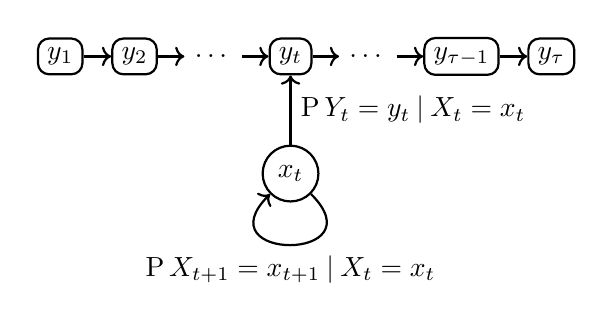
\begin{tikzpicture}[x=1pt,y=1pt]
        \matrix [column sep=10] {
            \node [box] (e1) {$y_1$}; & \node [box] (e2) {$y_2$}; & \node [box,draw=none] (da) {$\dots$}; & \node [box] (et) {$y_t$}; & \node [box,draw=none] (db) {$\dots$}; & \node [box] (etauprev) {$y_{\tau - 1}$}; & \node [box] (etau) {$y_\tau$}; \\
        };
        \node [box,circle,below=25 of et] (st) {$x_t$};
        \draw [->,thick] (e1) -- (e2);
        \draw [->,thick] (e2) -- (da);
        \draw [->,thick] (da) -- (et);
        \draw [->,thick] (et) -- (db);
        \draw [->,thick] (db) -- (etauprev);
        \draw [->,thick] (etauprev) -- (etau);
        \draw [->,thick] (st) -- (et) node[midway,right] {$\prob\pan{Y_t = y_t \giv X_t = x_t}$};
        \draw [->,thick] (st) to [loop,looseness=6,out=315,in=225] node[midway,below] {$\prob\pan{X_{t + 1} = x_{t+1} \giv X_t = x_t}$} (st);
    \end{tikzpicture}
\end{figure}

\subsection{Interleaved HMM}\label{sec:interleaved_hmm}

While a single HMM can intuitively model a single process, A software system often comprises multiple processes. For example, a single system might run multiple programs, each utilizing multiple threads. Furthermore, event logs from each process may be collected and gathered in a centralized storage. 

Individual threads can also communicate with each other, possibly across different hardware. Thus, data flows across thread boundaries. In this case, processes may not be restricted to a single thread. Instead, it is more suitable to let the hidden states model the states of the data flow of the whole system.

Following this parallel computation paradigm, we can mix multiple HMMs. This mixture of HMMs can be encoded into a single HMM, called \emph{interleaved HMM}\cite{Minot2014-gn}. All constituent hidden Markov chains produce observation events in the same sequence, but at any time step, only one individual chain can transition as dictated by some random process \(C\).

Consider the random variable \(X_t\) for a state at type \(t\). It can be defined as composition of states of \(m\) different HMMs \(\mu_k\) for \(1 \leq k \leq m\):
\begin{equation}\label{eq:state_encoding}
    X_t = \pan{S_{\mu_1,t}, S_{\mu_2,t}, ..., S_{\mu_m,t}, C_t}.
\end{equation}
\(C_t\) is a random variable used to index which chain is allowed to transition. It can be defined in different ways, including as an observation of another additional HMM, but for simplicity and following the fact that interleaving in even logs is mostly random, we choose that
\begin{equation}
    \alpha_c = \prob\pan{C_t = c}.
\end{equation}
where \(\alpha_c\) is a scalar probability representing the rate at which a chain is chosen. Intuitively, it is the probability that the underlying process of the constituent chain is chosen to generate an event. The new states of the interleaved HMM encode the state of all the constituent HMM using indexing tricks, as shown in \cite{Minot2014-gn}.

At any time \(t\), the probability of the constituent chain \(\mu\) to transition from state \(s\) to \(s'\) is then
\begin{equation}
    \prob\pan{S_{\mu,t+1} = s' \giv S_{\mu,t} = s, C_t = c_t} = \begin{cases}
        a_{\mu,s,s'} & \text{if $c_t = \mu$,} \\
        \delta\pan{s, s'} & \text{otherwise,} \\
    \end{cases}
\end{equation}
where \(\delta\) is the indicator function.
Then, \cref{eq:transition,eq:prior,eq:emission} are redefined as follows:
\begin{equation}\label{eq:interleaved_transition}
    \begin{multlined}
        a_{x_{t+1}, x_t} =
        \alpha_{c_t}\prod_{\mu} \prob\pan{S_{\mu,t+1} = s_{\mu,t+1} \giv S_{\mu,t} = s_{\mu,t}, C_t = c_t},
    \end{multlined}
\end{equation}
\begin{equation}
    \pi_x = \alpha_c \prod_\mu \pi_{\mu,s_\mu},
\end{equation}
and
\begin{equation}
    b_{x,y} = b_{c,s_c,y}
\end{equation}
\Cref{eq:state_encoding,eq:interleaved_transition} indicates an explosion of states. Indeed, we discuss in detail how this impacts the model's training and possible remedies in \cref{sec:approach}. Nonetheless, we will see in \cref{sec:results} that a smaller model might be more desirable in line with the findings of \cite{Cohen2005-mn}.

\section{Approach}\label{sec:approach}

We propose an automatic workload generation approach that leverages generative models and their unsupervised learning capabilities. Similar to \cite{Yadwadkar2010-ml}, we use a mixture of HMM. We use the interleaved HMM described in \cref{sec:interleaved_hmm}. We first extract sequences of actions that will constitute a workload. We use event logs as a proxy, as they are widely available, capture user behavior, and are relatively less complex to maintain than directly captured user inputs.

In this approach, only a small set of user actions must be collected to train the model. Once fitted, the model can extrapolate realistic synthetic workloads with high entropy.

Unlike \cite{Chen2019-fu}, we do not consider clusters of users. As event logs are noisy and does not contain enough user identifiers \cite{Zhao2023-nh} to relate actions to users. Instead, we rely on the fact that the interleaved HMM will eventually learn distinct patterns and behaviors in different constituent chains.

%todo a visualization of the steps

\subsection{Collection Action Sequences}

The first step in our approach is collecting action sequences. Traditionally, actions are obtained by collecting user inputs, after which they are organized into workflows. However, as pointed out in \cite{Chen2019-fu}, this method is not cost-efficient and often times impractical due to the size and heterogeneity of large software systems.

Following the approach of \cite{Chen2019-fu}, we use event logs as a proxy to user inputs to mirror the user behaviors. Logs also contain system behavior information that is not present in user inputs. This way, we can model the user behaviors and their interaction with different subsystems.

One caveat is that collecting actions from logs requires manual intervention. Once actions have been identified in logs, they need to be manually implemented to be replayed for load testing.

\subsection{Fitting a HMM}

Once we have a dataset of action sequences, it is used to train an interleaved HMM. In the context of Markov chains, actions are observed events.
The traditional algorithm still applies to interleaved HMMs since they are merely regular HMMs encoding the states and probabilities of multiple constituent chains.

Consider a HMM \(\mu\) with state sequence \(\seq{X_1, X_2, ..., X_\tau}\) and an event sequence \(\seq{Y_1, Y_2, ..., Y_\tau}\). To fit this HMM on a hidden process, we need to find parameters \(a, b\) and \(\pi\) of \(mu\), by maximizing the likelihood \(\mathcal{L}(\mu | \seq{Y_t = y_t}_{t=1}^\tau)\). For some observed events \(\seq{y_1, y_2, ..., y_\tau}\), it can be written as
\begin{equation}\label{eq:likelihood}
    \begin{aligned}
        \mathcal{L}(\mu | \seq{Y_t = y_t}_{t=1}^\tau)
        &= \prob\pan{\seq{Y_t = y_t}_{t=1}^\tau}. \\
        &= \sum_{x_\tau} \prob\pan*{\seq{Y_t = y_t}_{t=1}^{\tau} \:,\: X_\tau = x_\tau}
    \end{aligned}
\end{equation}
Let \(p_\mu\pan{\seq{y_t}_{t=1}^{\tau} \:,\: x_\tau} = \prob\pan*{\seq{Y_t = y_t}_{t=1}^{\tau} \:,\: X_\tau = x_\tau}\).
By recursively applying the chain rule that for \(1
\leq t \leq \tau\)
\begin{equation}\label{eq:forward}
    \begin{multlined}
        p_\mu\pan{\seq{y_t}_{t=1}^{\tau} \:,\: x_\tau} = \\
        b_{x_\tau,y_\tau} \sum_{x_{\tau-1}} a_{x_{\tau}, x_{\tau-1}} p_\mu\pan{\seq{y_t}_{t=0}^{\tau-1}\:,\: x_{\tau-1}}.
    \end{multlined}
\end{equation}
and with the base case
\begin{equation}\label{eq:forward_base}
    p_\mu\pan{\seq{} \:,\: x_0} = \prob\pan{X_0 = x_0}.
\end{equation}

Using \cref{eq:likelihood,eq:forward,eq:forward_base} we can construct \cref{alg:forward}, the forward algorithm, to compute the likelihood. First, we initialize for all states \(x\) a prior probability \(p_x\). Second, we iteratively update \(p_x\) using \cref{eq:forward}. Finally, the likelihood is obtained by taking the sum for all states according to \cref{eq:likelihood}.

\begin{algorithm}
    \caption{The forward algorithm. It computes the likelihood using \cref{eq:likelihood,eq:forward,eq:forward_base}.}\label{alg:forward}
    \begin{algorithmic}[1]
        \Procedure{Forward}{$\seq{y_t}_{t=1}^\tau$}
            \For{$x \gets \mathcal{S}$}
                \State $p_x \gets \pi_i$
            \EndFor
            \For{$t \gets \set{1, 2, ..., \tau}$}
                \For{$x' \gets \mathcal{S}$}
                    \State $p_{x'} \gets b_{x',y_t} \sum_{x \in \mathcal{S}} p_x a_{x, x'}$
                \EndFor
            \EndFor
            \State \Return $\sum_{x \in \mathcal{S}} p_x$
        \EndProcedure
    \end{algorithmic}
\end{algorithm}

Then, the fitted model \(\hat{\mu}\) is one that maximizes the likehood:
\begin{equation}
    \label{eq:max_likelihood}
    \hat{\mu} = \argmax_{\mu} \mathcal{L}\pan{\mu \giv \seq{Y_t = y_t}_{t=1}^\tau}.
\end{equation}

Since the forward algorithm's gradient can be automatically computed by auto differentiation frameworks such as Jax\cite{Bradbury2018-jz}, \cref{eq:max_likelihood} can be solved using stochastic gradient descent algorithms instead of the traditional expectation maximization algorithm\cite{Minot2014-gn}. Specifically, I used the Adam\cite{Kingma2014-jj} optimizer on a synthetic dataset described in \cref{sec:dataset}. I implemented the forward algorithm in \(\log\) space for better numerical stability, and thus, the loss to be minimized is the negative log-likelihood:
\begin{equation}
    \label{eq:neg_log_likelihood}
    l = - \log \mathcal{L}\pan{\mu \giv \seq{Y_t = y_t}_{t=1}^\tau}.
\end{equation}

The forward algorithm has space complexity \(O(n)\)  and time complexity \(O(nT)\) where \(n\) is the number of possible states and \(T\) is the length of the input sequence. In the context of interleaved HMM \(\mu\), there are \(K\) individual HMMs \(\mu_k\), the state of \(\mu\) must encode the states of all \(\mu_k\). Thus, no matter the encoding, the time and space complexity of the forward algorithm will be exponential with respect to \(K\). Training the interleaved HMM is an intractable problem\cite{Landwehr2008-vw}. However, we find in \cref{sec:results} that a small model is enough to generate adequate workloads.

\subsection{Generating Workloads}

Once the model has been trained, we can use it to generate workloads one action at a time. There are many ways we can generate. One way is to iteratively select single constituent chains and apply \cref{alg:generate} on each to produce separated action sequences. However, the method we adopt instead is to apply \cref{alg:generate} directly to the interleaved HMM to obtain a sequence of interleaved actions as the whole workflow. Intuitively, this is closer to how multiple user inputs interact in real workloads.

\Cref{alg:generate} takes an initial state \(x\) and a desired sequence length \(\tau\). It iteratively updates \(x\) by calling a random choice function with weights given by the transition probabilities \(a\). This corresponds to the transition step. After each transition, an action is chosen to be emitted using the same random choice function, this time with weights given by emission probabilities \(b\).

\begin{algorithm}
    \caption{Generates a sequence of actions}\label{alg:generate}
    \begin{algorithmic}[1]
        \Procedure{Generate}{$x, \tau$}
            \For{$t \in \set{1, 2, ..., \tau}$}
                \State $x \gets$ \Call{Choose}{$\mathcal{S}, a_x$}
                \State $y_t \gets$ \Call{Choose}{$\mathcal{O}, b_x$}
            \EndFor
            \State \Return $\seq{y_1, y_2, ..., y_\tau}$
        \EndProcedure
    \end{algorithmic}
\end{algorithm}

\section{Experimental Setup}\label{sec:experimental_setup}

We have implemented the interleaved HMM using the Flax\cite{Heek2023-nl} framework based on Jax\cite{Bradbury2018-jz}. To achieve better numerical stability, \cref{alg:forward,alg:generate} are implemented in log space.
We evaluate two variants of our approach.

With the first variant, which we call \worklogalpha{}, we train an interleaved HMM directly using \cref{alg:forward}. The number of subchains and states it are both limited to 4 to reduce computation overhead.

Alternatively, with the second variant, \worklogbeta{}, we train each constituent chains separately using \cref{alg:forward}. Although computationally more efficient, it is the worst approximation.

\subsection{Research Questions}

\begin{researchquestions}
    \item\label{rq:performance} \emph{How does our approach perform for real workloads?} Can we say that our approach can produce realistic workloads? In practice, while HMMs can naturally model stochastic processes, the model might not be accurate due to the limitation in the number of states. Thus, we investigate the realism versus variance tradeoff.
    \item\label{rq:ablation} \emph{How does the approach perform under different settings?} Due to the many tunable parameters and workload characteristics, that is, the number of constituent chains in the interleaved HMM, the number of states in each chain, the number of actions, and the training batch sizes, it is important to know which configuration yields better results.
\end{researchquestions}

\subsection{Evaluation Metrics}

We use two different metrics to evaluate the realism and randomness of each variant of our approach.

\subsubsection{Throughput Delta}

The first metric is Cliff's delta\cite{Cohen2013-up,Cliff1993-he} of the \emph{throughput} of the actual action sequence against that of generated action sequences. We define throughput as
\begin{equation}
    \prob\pan{\seq{Y_t = y}_{t=1}^\tau}
\end{equation}
for a specific action \(y\). Following suggestions from \cite{Sawilowsky2009-oy}, we use the following interpretation of Cliff's delta:
\(\approx 0.01\) indicates a very small difference, \(\approx 0.2\) is small, \(\approx 0.5\) is medium, \(\approx 0.8\) is large, \(\approx 1.2\) is very large and \(\approx 2\) is huge.

\subsubsection{Perplexity}

Using the negative log-likelihood as a cross-entropy, we define \emph{perplexity} as
\begin{equation}
    \prob\pan{\seq{Y_t = y_t}_{t=0}^{\tau}}^{-\frac{1}{\tau}}
\end{equation}
for a sequence of observation \(\seq{y_t}_{t=0}^\tau\). Because the interpretation of this metric is relative to the model, we only use this metric to compare a model against variants of itself. Usually, for example, with language models, perplexity can be interpreted as the model's randomness and confusion. However, we adapt this metric to measure the randomness of the generated workloads. Thus, higher is better.

\subsection{Datasets}\label{sec:dataset}

We use both datasets from real software projects and synthetically generated datasets.

\subsubsection{Real Datasets}

To answer \cref{rq:performance}, we use datasets taken from \cite{Chen2019-fu}. They consist of data from two open-source projects, Apache James and OpenMRS, and one industrial project, Google Borg.

Apache James is an enterprise mail server. \cite{Chen2019-fu} used JMeter to generate a workload of around 2000 users and captured its log. Only two types of actions are considered: ``SEND,'' where a user sends an email, and ``RECEIVE,'' where a user receives and loads an email.

OpenMRS is a web medical record service. \cite{Chen2019-fu} used the default demo database with over 5000 patients and 476,000 user actions. Four action types are considered: ``ADD'', ``DELETE'', ``SEARCH'' and ``EDIT''. They used JMeter and injected more randomness to simulate a more realistic workload.

\subsubsection{Synthetic Datasets}

To answer \cref{rq:ablation}, we use a synthetic dataset, which we generate using a hardcoded interleaved HMM. The parameters of the HMM used to generate the dataset are not shared with the HMM under evaluation. Since the model is stochastic, it will not learn the same parameters as the HMM used to generate the dataset. By varying the parameters of the hardcoded HMM, we can obtain synthetic datasets with different characteristics, which we leverage to reveal insights about the variants of our approach.

In our experimentation, we use a small sample of approximately 1000 actions for each dataset. 90\% of each dataset is used to train the model, while 10\% is used for evaluation. That is, our model is evaluated on unseen data.

\section{Results}\label{sec:results}

\subsection*{\cref{rq:performance}: How does our approach perform for real workloads?}

\begin{table}
\caption{Throughput delta on the Apache James dataset.}\label{tab:throughput_apache_james}
\begin{tabular}{@{}l|l|lll@{}}
\toprule
\multicolumn{4}{c}{Apache James}                         \\ \midrule
        & throughput & \worklogalpha   & \worklogbeta    \\ \midrule
SEND    & 2.746      & \textbf{0.0322} & 0.0835          \\
RECEIVE & 7.254      & \textbf{0.0322} & 0.0835          \\ \midrule
Mean    & 5.000      & \textbf{0.0322} & 0.0835          \\ \bottomrule
\end{tabular}
\end{table}

\begin{table}
\caption{Throughput delta on the OpenMRS dataset.}\label{tab:throughput_openmrs}
\begin{tabular}{@{}l|l|lll@{}}
\toprule
\multicolumn{4}{c}{OpenMRS}                         \\ \midrule
       & throughput & \worklogalpha   & \worklogbeta    \\ \midrule
ADD    & 2.848      & \textbf{0.0163} & 0.0631          \\
DELETE & 3.080      & 0.0285          & \textbf{0.0151} \\
EXIT   & 2.066      & 0.0395          & \textbf{0.0305} \\
SEARCH & 2.006      & \textbf{0.0035} & 0.0374          \\ \midrule
Mean   & 2.500      & \textbf{0.0220} & 0.0365          \\ \bottomrule
\end{tabular}
\end{table}

\begin{table}
\caption{Throughput delta on the Google Borg dataset.}\label{tab:throughput_google_borg}
\begin{tabular}{@{}l|l|ll@{}}
\toprule
\multicolumn{4}{c}{Google Borg}                         \\ \midrule
         & throughput & \worklogalpha   & \worklogbeta    \\ \midrule
SUBMIT   & 3.453      & 0.0447          & \textbf{0.0423} \\
SCHEDULE & 1.009      & \textbf{0.0529} & 0.2128          \\
FAIL     & 0.398      & \textbf{0.0978} & 0.2230          \\
FINISH   & 3.472      & \textbf{0.0984} & 0.1286          \\
EVICT    & 1.636      & \textbf{0.0459} & 0.1282          \\
KILL     & 0.032      & 0.0060          & \textbf{0.0010} \\ \midrule
Mean     & 1.667      & \textbf{0.0576} & 0.1228          \\ \bottomrule
\end{tabular}
\end{table}

To answer this question, we evaluated \worklogalpha{} and \worklogbeta{} against Apache James, OpenMRS, and Google Borg datasets. For each dataset, we train a new interleaved HMM, each configured with the correct number of action types. Then, we generate a matching amount of sequences. Finally, for each action type, we compute the Cliff's delta of the throughput of sequences from the original dataset against the throughput of generated sequences.

We present the results in \cref{tab:throughput_apache_james,tab:throughput_openmrs,tab:throughput_google_borg}. Overall, \worklogalpha{} seems to perform better than \worklogbeta{}. This is expected due to the fact that \worklogbeta{} uses an approximation of \cref{alg:forward} during training. However, we note that \worklogbeta{} is an order of magnitude faster to train. 

Both \worklogalpha{} and \worklogbeta{} perform well on the Apache James dataset, with very small deltas and with \worklogalpha{} performing slightly better than \worklogbeta{}. Coincidentally, the models have a constant delta for both types of actions, potentially indicating that both models learned as many user behavior patterns as their randomness would allow.

On the OpenMRS dataset, the difference in throughput delta between the two variants starts to blur. For the ``ADD'' and ``SEARCH'' action types, \worklogalpha{} performs slightly better, whereas for the ``DELETE'' and ``EXIT'' action types, \worklogbeta{} is better.

This is because users behave differently for different actions, and \worklogbeta{} learns some patterns faster. In \cref{tab:throughput_google_borg} is where we see \worklogbeta{} starts to struggle. \worklogalpha{} performs better for all action types except for ``SUBMIT'' and ``KILL''. On this dataset, \worklogbeta{} has a larger but still small delta.

\emph{Finding 1: Overall, both variants can reproduce realistic workloads. \worklogalpha{} performs slightly better on larger datasets.}

\subsection*{\cref{rq:ablation}: How does our approach perform under different settings?}

\begin{table}
\caption{Performance of \worklogalpha{} and \worklogbeta{} on synthetic datasets. ``Delta'' is the Cliff's delta of the throughput.}\label{tab:ablation_dataset}
\begin{tabular}{@{}l|ll|ll@{}}
\toprule
     & \multicolumn{2}{c|}{\worklogalpha} & \multicolumn{2}{c}{\worklogbeta} \\ \midrule
     & delta           & perplexity      & delta           & perplexity      \\ \midrule
Easy & \textbf{0.0304} & 3.6973          & 0.0601          & \textbf{14.916} \\
Wide & \textbf{0.0311} & 3.9588          & 0.1025          & \textbf{15.919} \\
Hard & 0.7370          & 4.1623          & \textbf{0.7364} & \textbf{16.123} \\ \bottomrule
\end{tabular}
\end{table}

To answer this question, we first evaluate both \worklogalpha{} and \worklogbeta{} on three different configurations of our synthetic dataset. We train a new model for each dataset instance and measure both the throughput delta and the perplexity.

The easy dataset is generated by an interleaved HMM with 4 constituent chains of 4 states each. The wide dataset is generated by an interleaved HMM with 16 constituent chains of 4 states each. The hard dataset is generated by an interleaved HMM with 4 constituent chains of 16 states each.

The results are recorded in \cref{tab:ablation_dataset}. We can observe that both variants produce sequences that are more realistic, e.g., have a smaller throughput delta, on datasets with a smaller number of underlying states. They struggle to reproduce the hard dataset, which has a higher number of underlying states. The number of constituent chains seems to not have an influence on the performance of \worklogalpha{}, as indicated by the wide dataset. We also note that, overall, \worklogbeta{} has higher perplexity, indicating more randomness.

\emph{Finding 2: Both variants struggle when the number of underlying states are increased. \worklogbeta{} can produce more random sequences.}

\begin{figure}
    \caption{Performance of \worklogbeta{} versus number of constituent chains.}\label{fig:ablation_wide}
    \centering
    \begin{subfigure}{.5\columnwidth}
        \caption{throughput delta}
        \centering
        \resizebox{\textwidth}{!}{%% Creator: Matplotlib, PGF backend
%%
%% To include the figure in your LaTeX document, write
%%   \input{<filename>.pgf}
%%
%% Make sure the required packages are loaded in your preamble
%%   \usepackage{pgf}
%%
%% Also ensure that all the required font packages are loaded; for instance,
%% the lmodern package is sometimes necessary when using math font.
%%   \usepackage{lmodern}
%%
%% Figures using additional raster images can only be included by \input if
%% they are in the same directory as the main LaTeX file. For loading figures
%% from other directories you can use the `import` package
%%   \usepackage{import}
%%
%% and then include the figures with
%%   \import{<path to file>}{<filename>.pgf}
%%
%% Matplotlib used the following preamble
%%   \def\mathdefault#1{#1}
%%   \everymath=\expandafter{\the\everymath\displaystyle}
%%   
%%   \usepackage{fontspec}
%%   \setmainfont{DejaVuSerif.ttf}[Path=\detokenize{/Users/boluo/Library/Application Support/hatch/env/virtual/worklog/d3HGslSU/worklog/lib/python3.11/site-packages/matplotlib/mpl-data/fonts/ttf/}]
%%   \setsansfont{DejaVuSans.ttf}[Path=\detokenize{/Users/boluo/Library/Application Support/hatch/env/virtual/worklog/d3HGslSU/worklog/lib/python3.11/site-packages/matplotlib/mpl-data/fonts/ttf/}]
%%   \setmonofont{DejaVuSansMono.ttf}[Path=\detokenize{/Users/boluo/Library/Application Support/hatch/env/virtual/worklog/d3HGslSU/worklog/lib/python3.11/site-packages/matplotlib/mpl-data/fonts/ttf/}]
%%   \makeatletter\@ifpackageloaded{underscore}{}{\usepackage[strings]{underscore}}\makeatother
%%
\begingroup%
\makeatletter%
\begin{pgfpicture}%
\pgfpathrectangle{\pgfpointorigin}{\pgfqpoint{1.923967in}{1.930603in}}%
\pgfusepath{use as bounding box, clip}%
\begin{pgfscope}%
\pgfsetbuttcap%
\pgfsetmiterjoin%
\definecolor{currentfill}{rgb}{1.000000,1.000000,1.000000}%
\pgfsetfillcolor{currentfill}%
\pgfsetlinewidth{0.000000pt}%
\definecolor{currentstroke}{rgb}{1.000000,1.000000,1.000000}%
\pgfsetstrokecolor{currentstroke}%
\pgfsetdash{}{0pt}%
\pgfpathmoveto{\pgfqpoint{0.000000in}{0.000000in}}%
\pgfpathlineto{\pgfqpoint{1.923967in}{0.000000in}}%
\pgfpathlineto{\pgfqpoint{1.923967in}{1.930603in}}%
\pgfpathlineto{\pgfqpoint{0.000000in}{1.930603in}}%
\pgfpathlineto{\pgfqpoint{0.000000in}{0.000000in}}%
\pgfpathclose%
\pgfusepath{fill}%
\end{pgfscope}%
\begin{pgfscope}%
\pgfsetbuttcap%
\pgfsetmiterjoin%
\definecolor{currentfill}{rgb}{1.000000,1.000000,1.000000}%
\pgfsetfillcolor{currentfill}%
\pgfsetlinewidth{0.000000pt}%
\definecolor{currentstroke}{rgb}{0.000000,0.000000,0.000000}%
\pgfsetstrokecolor{currentstroke}%
\pgfsetstrokeopacity{0.000000}%
\pgfsetdash{}{0pt}%
\pgfpathmoveto{\pgfqpoint{0.506467in}{0.521603in}}%
\pgfpathlineto{\pgfqpoint{1.823967in}{0.521603in}}%
\pgfpathlineto{\pgfqpoint{1.823967in}{1.830603in}}%
\pgfpathlineto{\pgfqpoint{0.506467in}{1.830603in}}%
\pgfpathlineto{\pgfqpoint{0.506467in}{0.521603in}}%
\pgfpathclose%
\pgfusepath{fill}%
\end{pgfscope}%
\begin{pgfscope}%
\pgfsetbuttcap%
\pgfsetroundjoin%
\definecolor{currentfill}{rgb}{0.000000,0.000000,0.000000}%
\pgfsetfillcolor{currentfill}%
\pgfsetlinewidth{0.803000pt}%
\definecolor{currentstroke}{rgb}{0.000000,0.000000,0.000000}%
\pgfsetstrokecolor{currentstroke}%
\pgfsetdash{}{0pt}%
\pgfsys@defobject{currentmarker}{\pgfqpoint{0.000000in}{-0.048611in}}{\pgfqpoint{0.000000in}{0.000000in}}{%
\pgfpathmoveto{\pgfqpoint{0.000000in}{0.000000in}}%
\pgfpathlineto{\pgfqpoint{0.000000in}{-0.048611in}}%
\pgfusepath{stroke,fill}%
}%
\begin{pgfscope}%
\pgfsys@transformshift{0.823009in}{0.521603in}%
\pgfsys@useobject{currentmarker}{}%
\end{pgfscope}%
\end{pgfscope}%
\begin{pgfscope}%
\definecolor{textcolor}{rgb}{0.000000,0.000000,0.000000}%
\pgfsetstrokecolor{textcolor}%
\pgfsetfillcolor{textcolor}%
\pgftext[x=0.823009in,y=0.424381in,,top]{\color{textcolor}{\sffamily\fontsize{10.000000}{12.000000}\selectfont\catcode`\^=\active\def^{\ifmmode\sp\else\^{}\fi}\catcode`\%=\active\def%{\%}10}}%
\end{pgfscope}%
\begin{pgfscope}%
\pgfsetbuttcap%
\pgfsetroundjoin%
\definecolor{currentfill}{rgb}{0.000000,0.000000,0.000000}%
\pgfsetfillcolor{currentfill}%
\pgfsetlinewidth{0.803000pt}%
\definecolor{currentstroke}{rgb}{0.000000,0.000000,0.000000}%
\pgfsetstrokecolor{currentstroke}%
\pgfsetdash{}{0pt}%
\pgfsys@defobject{currentmarker}{\pgfqpoint{0.000000in}{-0.048611in}}{\pgfqpoint{0.000000in}{0.000000in}}{%
\pgfpathmoveto{\pgfqpoint{0.000000in}{0.000000in}}%
\pgfpathlineto{\pgfqpoint{0.000000in}{-0.048611in}}%
\pgfusepath{stroke,fill}%
}%
\begin{pgfscope}%
\pgfsys@transformshift{1.250769in}{0.521603in}%
\pgfsys@useobject{currentmarker}{}%
\end{pgfscope}%
\end{pgfscope}%
\begin{pgfscope}%
\definecolor{textcolor}{rgb}{0.000000,0.000000,0.000000}%
\pgfsetstrokecolor{textcolor}%
\pgfsetfillcolor{textcolor}%
\pgftext[x=1.250769in,y=0.424381in,,top]{\color{textcolor}{\sffamily\fontsize{10.000000}{12.000000}\selectfont\catcode`\^=\active\def^{\ifmmode\sp\else\^{}\fi}\catcode`\%=\active\def%{\%}20}}%
\end{pgfscope}%
\begin{pgfscope}%
\pgfsetbuttcap%
\pgfsetroundjoin%
\definecolor{currentfill}{rgb}{0.000000,0.000000,0.000000}%
\pgfsetfillcolor{currentfill}%
\pgfsetlinewidth{0.803000pt}%
\definecolor{currentstroke}{rgb}{0.000000,0.000000,0.000000}%
\pgfsetstrokecolor{currentstroke}%
\pgfsetdash{}{0pt}%
\pgfsys@defobject{currentmarker}{\pgfqpoint{0.000000in}{-0.048611in}}{\pgfqpoint{0.000000in}{0.000000in}}{%
\pgfpathmoveto{\pgfqpoint{0.000000in}{0.000000in}}%
\pgfpathlineto{\pgfqpoint{0.000000in}{-0.048611in}}%
\pgfusepath{stroke,fill}%
}%
\begin{pgfscope}%
\pgfsys@transformshift{1.678529in}{0.521603in}%
\pgfsys@useobject{currentmarker}{}%
\end{pgfscope}%
\end{pgfscope}%
\begin{pgfscope}%
\definecolor{textcolor}{rgb}{0.000000,0.000000,0.000000}%
\pgfsetstrokecolor{textcolor}%
\pgfsetfillcolor{textcolor}%
\pgftext[x=1.678529in,y=0.424381in,,top]{\color{textcolor}{\sffamily\fontsize{10.000000}{12.000000}\selectfont\catcode`\^=\active\def^{\ifmmode\sp\else\^{}\fi}\catcode`\%=\active\def%{\%}30}}%
\end{pgfscope}%
\begin{pgfscope}%
\definecolor{textcolor}{rgb}{0.000000,0.000000,0.000000}%
\pgfsetstrokecolor{textcolor}%
\pgfsetfillcolor{textcolor}%
\pgftext[x=1.165217in,y=0.234413in,,top]{\color{textcolor}{\sffamily\fontsize{10.000000}{12.000000}\selectfont\catcode`\^=\active\def^{\ifmmode\sp\else\^{}\fi}\catcode`\%=\active\def%{\%}number of chains}}%
\end{pgfscope}%
\begin{pgfscope}%
\pgfsetbuttcap%
\pgfsetroundjoin%
\definecolor{currentfill}{rgb}{0.000000,0.000000,0.000000}%
\pgfsetfillcolor{currentfill}%
\pgfsetlinewidth{0.803000pt}%
\definecolor{currentstroke}{rgb}{0.000000,0.000000,0.000000}%
\pgfsetstrokecolor{currentstroke}%
\pgfsetdash{}{0pt}%
\pgfsys@defobject{currentmarker}{\pgfqpoint{-0.048611in}{0.000000in}}{\pgfqpoint{-0.000000in}{0.000000in}}{%
\pgfpathmoveto{\pgfqpoint{-0.000000in}{0.000000in}}%
\pgfpathlineto{\pgfqpoint{-0.048611in}{0.000000in}}%
\pgfusepath{stroke,fill}%
}%
\begin{pgfscope}%
\pgfsys@transformshift{0.506467in}{0.521603in}%
\pgfsys@useobject{currentmarker}{}%
\end{pgfscope}%
\end{pgfscope}%
\begin{pgfscope}%
\definecolor{textcolor}{rgb}{0.000000,0.000000,0.000000}%
\pgfsetstrokecolor{textcolor}%
\pgfsetfillcolor{textcolor}%
\pgftext[x=0.100000in, y=0.468842in, left, base]{\color{textcolor}{\sffamily\fontsize{10.000000}{12.000000}\selectfont\catcode`\^=\active\def^{\ifmmode\sp\else\^{}\fi}\catcode`\%=\active\def%{\%}0.00}}%
\end{pgfscope}%
\begin{pgfscope}%
\pgfsetbuttcap%
\pgfsetroundjoin%
\definecolor{currentfill}{rgb}{0.000000,0.000000,0.000000}%
\pgfsetfillcolor{currentfill}%
\pgfsetlinewidth{0.803000pt}%
\definecolor{currentstroke}{rgb}{0.000000,0.000000,0.000000}%
\pgfsetstrokecolor{currentstroke}%
\pgfsetdash{}{0pt}%
\pgfsys@defobject{currentmarker}{\pgfqpoint{-0.048611in}{0.000000in}}{\pgfqpoint{-0.000000in}{0.000000in}}{%
\pgfpathmoveto{\pgfqpoint{-0.000000in}{0.000000in}}%
\pgfpathlineto{\pgfqpoint{-0.048611in}{0.000000in}}%
\pgfusepath{stroke,fill}%
}%
\begin{pgfscope}%
\pgfsys@transformshift{0.506467in}{1.045203in}%
\pgfsys@useobject{currentmarker}{}%
\end{pgfscope}%
\end{pgfscope}%
\begin{pgfscope}%
\definecolor{textcolor}{rgb}{0.000000,0.000000,0.000000}%
\pgfsetstrokecolor{textcolor}%
\pgfsetfillcolor{textcolor}%
\pgftext[x=0.100000in, y=0.992442in, left, base]{\color{textcolor}{\sffamily\fontsize{10.000000}{12.000000}\selectfont\catcode`\^=\active\def^{\ifmmode\sp\else\^{}\fi}\catcode`\%=\active\def%{\%}0.05}}%
\end{pgfscope}%
\begin{pgfscope}%
\pgfsetbuttcap%
\pgfsetroundjoin%
\definecolor{currentfill}{rgb}{0.000000,0.000000,0.000000}%
\pgfsetfillcolor{currentfill}%
\pgfsetlinewidth{0.803000pt}%
\definecolor{currentstroke}{rgb}{0.000000,0.000000,0.000000}%
\pgfsetstrokecolor{currentstroke}%
\pgfsetdash{}{0pt}%
\pgfsys@defobject{currentmarker}{\pgfqpoint{-0.048611in}{0.000000in}}{\pgfqpoint{-0.000000in}{0.000000in}}{%
\pgfpathmoveto{\pgfqpoint{-0.000000in}{0.000000in}}%
\pgfpathlineto{\pgfqpoint{-0.048611in}{0.000000in}}%
\pgfusepath{stroke,fill}%
}%
\begin{pgfscope}%
\pgfsys@transformshift{0.506467in}{1.568803in}%
\pgfsys@useobject{currentmarker}{}%
\end{pgfscope}%
\end{pgfscope}%
\begin{pgfscope}%
\definecolor{textcolor}{rgb}{0.000000,0.000000,0.000000}%
\pgfsetstrokecolor{textcolor}%
\pgfsetfillcolor{textcolor}%
\pgftext[x=0.100000in, y=1.516042in, left, base]{\color{textcolor}{\sffamily\fontsize{10.000000}{12.000000}\selectfont\catcode`\^=\active\def^{\ifmmode\sp\else\^{}\fi}\catcode`\%=\active\def%{\%}0.10}}%
\end{pgfscope}%
\begin{pgfscope}%
\pgfpathrectangle{\pgfqpoint{0.506467in}{0.521603in}}{\pgfqpoint{1.317500in}{1.309000in}}%
\pgfusepath{clip}%
\pgfsetrectcap%
\pgfsetroundjoin%
\pgfsetlinewidth{1.505625pt}%
\definecolor{currentstroke}{rgb}{0.121569,0.466667,0.705882}%
\pgfsetstrokecolor{currentstroke}%
\pgfsetdash{}{0pt}%
\pgfpathmoveto{\pgfqpoint{0.566353in}{1.151421in}}%
\pgfpathlineto{\pgfqpoint{0.737457in}{1.024170in}}%
\pgfpathlineto{\pgfqpoint{1.079665in}{1.205490in}}%
\pgfpathlineto{\pgfqpoint{1.764081in}{1.094461in}}%
\pgfusepath{stroke}%
\end{pgfscope}%
\begin{pgfscope}%
\pgfsetrectcap%
\pgfsetmiterjoin%
\pgfsetlinewidth{0.803000pt}%
\definecolor{currentstroke}{rgb}{0.000000,0.000000,0.000000}%
\pgfsetstrokecolor{currentstroke}%
\pgfsetdash{}{0pt}%
\pgfpathmoveto{\pgfqpoint{0.506467in}{0.521603in}}%
\pgfpathlineto{\pgfqpoint{0.506467in}{1.830603in}}%
\pgfusepath{stroke}%
\end{pgfscope}%
\begin{pgfscope}%
\pgfsetrectcap%
\pgfsetmiterjoin%
\pgfsetlinewidth{0.803000pt}%
\definecolor{currentstroke}{rgb}{0.000000,0.000000,0.000000}%
\pgfsetstrokecolor{currentstroke}%
\pgfsetdash{}{0pt}%
\pgfpathmoveto{\pgfqpoint{1.823967in}{0.521603in}}%
\pgfpathlineto{\pgfqpoint{1.823967in}{1.830603in}}%
\pgfusepath{stroke}%
\end{pgfscope}%
\begin{pgfscope}%
\pgfsetrectcap%
\pgfsetmiterjoin%
\pgfsetlinewidth{0.803000pt}%
\definecolor{currentstroke}{rgb}{0.000000,0.000000,0.000000}%
\pgfsetstrokecolor{currentstroke}%
\pgfsetdash{}{0pt}%
\pgfpathmoveto{\pgfqpoint{0.506467in}{0.521603in}}%
\pgfpathlineto{\pgfqpoint{1.823967in}{0.521603in}}%
\pgfusepath{stroke}%
\end{pgfscope}%
\begin{pgfscope}%
\pgfsetrectcap%
\pgfsetmiterjoin%
\pgfsetlinewidth{0.803000pt}%
\definecolor{currentstroke}{rgb}{0.000000,0.000000,0.000000}%
\pgfsetstrokecolor{currentstroke}%
\pgfsetdash{}{0pt}%
\pgfpathmoveto{\pgfqpoint{0.506467in}{1.830603in}}%
\pgfpathlineto{\pgfqpoint{1.823967in}{1.830603in}}%
\pgfusepath{stroke}%
\end{pgfscope}%
\end{pgfpicture}%
\makeatother%
\endgroup%
}
    \end{subfigure}%
    \begin{subfigure}{.5\columnwidth}
        \caption{perplexity}
        \centering
        \resizebox{0.97\textwidth}{!}{%% Creator: Matplotlib, PGF backend
%%
%% To include the figure in your LaTeX document, write
%%   \input{<filename>.pgf}
%%
%% Make sure the required packages are loaded in your preamble
%%   \usepackage{pgf}
%%
%% Also ensure that all the required font packages are loaded; for instance,
%% the lmodern package is sometimes necessary when using math font.
%%   \usepackage{lmodern}
%%
%% Figures using additional raster images can only be included by \input if
%% they are in the same directory as the main LaTeX file. For loading figures
%% from other directories you can use the `import` package
%%   \usepackage{import}
%%
%% and then include the figures with
%%   \import{<path to file>}{<filename>.pgf}
%%
%% Matplotlib used the following preamble
%%   \def\mathdefault#1{#1}
%%   \everymath=\expandafter{\the\everymath\displaystyle}
%%   
%%   \usepackage{fontspec}
%%   \setmainfont{DejaVuSerif.ttf}[Path=\detokenize{/Users/boluo/Library/Application Support/hatch/env/virtual/worklog/d3HGslSU/worklog/lib/python3.11/site-packages/matplotlib/mpl-data/fonts/ttf/}]
%%   \setsansfont{DejaVuSans.ttf}[Path=\detokenize{/Users/boluo/Library/Application Support/hatch/env/virtual/worklog/d3HGslSU/worklog/lib/python3.11/site-packages/matplotlib/mpl-data/fonts/ttf/}]
%%   \setmonofont{DejaVuSansMono.ttf}[Path=\detokenize{/Users/boluo/Library/Application Support/hatch/env/virtual/worklog/d3HGslSU/worklog/lib/python3.11/site-packages/matplotlib/mpl-data/fonts/ttf/}]
%%   \makeatletter\@ifpackageloaded{underscore}{}{\usepackage[strings]{underscore}}\makeatother
%%
\begingroup%
\makeatletter%
\begin{pgfpicture}%
\pgfpathrectangle{\pgfpointorigin}{\pgfqpoint{1.879818in}{1.930603in}}%
\pgfusepath{use as bounding box, clip}%
\begin{pgfscope}%
\pgfsetbuttcap%
\pgfsetmiterjoin%
\definecolor{currentfill}{rgb}{1.000000,1.000000,1.000000}%
\pgfsetfillcolor{currentfill}%
\pgfsetlinewidth{0.000000pt}%
\definecolor{currentstroke}{rgb}{1.000000,1.000000,1.000000}%
\pgfsetstrokecolor{currentstroke}%
\pgfsetdash{}{0pt}%
\pgfpathmoveto{\pgfqpoint{0.000000in}{0.000000in}}%
\pgfpathlineto{\pgfqpoint{1.879818in}{0.000000in}}%
\pgfpathlineto{\pgfqpoint{1.879818in}{1.930603in}}%
\pgfpathlineto{\pgfqpoint{0.000000in}{1.930603in}}%
\pgfpathlineto{\pgfqpoint{0.000000in}{0.000000in}}%
\pgfpathclose%
\pgfusepath{fill}%
\end{pgfscope}%
\begin{pgfscope}%
\pgfsetbuttcap%
\pgfsetmiterjoin%
\definecolor{currentfill}{rgb}{1.000000,1.000000,1.000000}%
\pgfsetfillcolor{currentfill}%
\pgfsetlinewidth{0.000000pt}%
\definecolor{currentstroke}{rgb}{0.000000,0.000000,0.000000}%
\pgfsetstrokecolor{currentstroke}%
\pgfsetstrokeopacity{0.000000}%
\pgfsetdash{}{0pt}%
\pgfpathmoveto{\pgfqpoint{0.462318in}{0.521603in}}%
\pgfpathlineto{\pgfqpoint{1.779818in}{0.521603in}}%
\pgfpathlineto{\pgfqpoint{1.779818in}{1.830603in}}%
\pgfpathlineto{\pgfqpoint{0.462318in}{1.830603in}}%
\pgfpathlineto{\pgfqpoint{0.462318in}{0.521603in}}%
\pgfpathclose%
\pgfusepath{fill}%
\end{pgfscope}%
\begin{pgfscope}%
\pgfsetbuttcap%
\pgfsetroundjoin%
\definecolor{currentfill}{rgb}{0.000000,0.000000,0.000000}%
\pgfsetfillcolor{currentfill}%
\pgfsetlinewidth{0.803000pt}%
\definecolor{currentstroke}{rgb}{0.000000,0.000000,0.000000}%
\pgfsetstrokecolor{currentstroke}%
\pgfsetdash{}{0pt}%
\pgfsys@defobject{currentmarker}{\pgfqpoint{0.000000in}{-0.048611in}}{\pgfqpoint{0.000000in}{0.000000in}}{%
\pgfpathmoveto{\pgfqpoint{0.000000in}{0.000000in}}%
\pgfpathlineto{\pgfqpoint{0.000000in}{-0.048611in}}%
\pgfusepath{stroke,fill}%
}%
\begin{pgfscope}%
\pgfsys@transformshift{0.778860in}{0.521603in}%
\pgfsys@useobject{currentmarker}{}%
\end{pgfscope}%
\end{pgfscope}%
\begin{pgfscope}%
\definecolor{textcolor}{rgb}{0.000000,0.000000,0.000000}%
\pgfsetstrokecolor{textcolor}%
\pgfsetfillcolor{textcolor}%
\pgftext[x=0.778860in,y=0.424381in,,top]{\color{textcolor}{\sffamily\fontsize{10.000000}{12.000000}\selectfont\catcode`\^=\active\def^{\ifmmode\sp\else\^{}\fi}\catcode`\%=\active\def%{\%}10}}%
\end{pgfscope}%
\begin{pgfscope}%
\pgfsetbuttcap%
\pgfsetroundjoin%
\definecolor{currentfill}{rgb}{0.000000,0.000000,0.000000}%
\pgfsetfillcolor{currentfill}%
\pgfsetlinewidth{0.803000pt}%
\definecolor{currentstroke}{rgb}{0.000000,0.000000,0.000000}%
\pgfsetstrokecolor{currentstroke}%
\pgfsetdash{}{0pt}%
\pgfsys@defobject{currentmarker}{\pgfqpoint{0.000000in}{-0.048611in}}{\pgfqpoint{0.000000in}{0.000000in}}{%
\pgfpathmoveto{\pgfqpoint{0.000000in}{0.000000in}}%
\pgfpathlineto{\pgfqpoint{0.000000in}{-0.048611in}}%
\pgfusepath{stroke,fill}%
}%
\begin{pgfscope}%
\pgfsys@transformshift{1.206620in}{0.521603in}%
\pgfsys@useobject{currentmarker}{}%
\end{pgfscope}%
\end{pgfscope}%
\begin{pgfscope}%
\definecolor{textcolor}{rgb}{0.000000,0.000000,0.000000}%
\pgfsetstrokecolor{textcolor}%
\pgfsetfillcolor{textcolor}%
\pgftext[x=1.206620in,y=0.424381in,,top]{\color{textcolor}{\sffamily\fontsize{10.000000}{12.000000}\selectfont\catcode`\^=\active\def^{\ifmmode\sp\else\^{}\fi}\catcode`\%=\active\def%{\%}20}}%
\end{pgfscope}%
\begin{pgfscope}%
\pgfsetbuttcap%
\pgfsetroundjoin%
\definecolor{currentfill}{rgb}{0.000000,0.000000,0.000000}%
\pgfsetfillcolor{currentfill}%
\pgfsetlinewidth{0.803000pt}%
\definecolor{currentstroke}{rgb}{0.000000,0.000000,0.000000}%
\pgfsetstrokecolor{currentstroke}%
\pgfsetdash{}{0pt}%
\pgfsys@defobject{currentmarker}{\pgfqpoint{0.000000in}{-0.048611in}}{\pgfqpoint{0.000000in}{0.000000in}}{%
\pgfpathmoveto{\pgfqpoint{0.000000in}{0.000000in}}%
\pgfpathlineto{\pgfqpoint{0.000000in}{-0.048611in}}%
\pgfusepath{stroke,fill}%
}%
\begin{pgfscope}%
\pgfsys@transformshift{1.634380in}{0.521603in}%
\pgfsys@useobject{currentmarker}{}%
\end{pgfscope}%
\end{pgfscope}%
\begin{pgfscope}%
\definecolor{textcolor}{rgb}{0.000000,0.000000,0.000000}%
\pgfsetstrokecolor{textcolor}%
\pgfsetfillcolor{textcolor}%
\pgftext[x=1.634380in,y=0.424381in,,top]{\color{textcolor}{\sffamily\fontsize{10.000000}{12.000000}\selectfont\catcode`\^=\active\def^{\ifmmode\sp\else\^{}\fi}\catcode`\%=\active\def%{\%}30}}%
\end{pgfscope}%
\begin{pgfscope}%
\definecolor{textcolor}{rgb}{0.000000,0.000000,0.000000}%
\pgfsetstrokecolor{textcolor}%
\pgfsetfillcolor{textcolor}%
\pgftext[x=1.121068in,y=0.234413in,,top]{\color{textcolor}{\sffamily\fontsize{10.000000}{12.000000}\selectfont\catcode`\^=\active\def^{\ifmmode\sp\else\^{}\fi}\catcode`\%=\active\def%{\%}number of chains}}%
\end{pgfscope}%
\begin{pgfscope}%
\pgfsetbuttcap%
\pgfsetroundjoin%
\definecolor{currentfill}{rgb}{0.000000,0.000000,0.000000}%
\pgfsetfillcolor{currentfill}%
\pgfsetlinewidth{0.803000pt}%
\definecolor{currentstroke}{rgb}{0.000000,0.000000,0.000000}%
\pgfsetstrokecolor{currentstroke}%
\pgfsetdash{}{0pt}%
\pgfsys@defobject{currentmarker}{\pgfqpoint{-0.048611in}{0.000000in}}{\pgfqpoint{-0.000000in}{0.000000in}}{%
\pgfpathmoveto{\pgfqpoint{-0.000000in}{0.000000in}}%
\pgfpathlineto{\pgfqpoint{-0.048611in}{0.000000in}}%
\pgfusepath{stroke,fill}%
}%
\begin{pgfscope}%
\pgfsys@transformshift{0.462318in}{0.521603in}%
\pgfsys@useobject{currentmarker}{}%
\end{pgfscope}%
\end{pgfscope}%
\begin{pgfscope}%
\definecolor{textcolor}{rgb}{0.000000,0.000000,0.000000}%
\pgfsetstrokecolor{textcolor}%
\pgfsetfillcolor{textcolor}%
\pgftext[x=0.276731in, y=0.468842in, left, base]{\color{textcolor}{\sffamily\fontsize{10.000000}{12.000000}\selectfont\catcode`\^=\active\def^{\ifmmode\sp\else\^{}\fi}\catcode`\%=\active\def%{\%}0}}%
\end{pgfscope}%
\begin{pgfscope}%
\pgfsetbuttcap%
\pgfsetroundjoin%
\definecolor{currentfill}{rgb}{0.000000,0.000000,0.000000}%
\pgfsetfillcolor{currentfill}%
\pgfsetlinewidth{0.803000pt}%
\definecolor{currentstroke}{rgb}{0.000000,0.000000,0.000000}%
\pgfsetstrokecolor{currentstroke}%
\pgfsetdash{}{0pt}%
\pgfsys@defobject{currentmarker}{\pgfqpoint{-0.048611in}{0.000000in}}{\pgfqpoint{-0.000000in}{0.000000in}}{%
\pgfpathmoveto{\pgfqpoint{-0.000000in}{0.000000in}}%
\pgfpathlineto{\pgfqpoint{-0.048611in}{0.000000in}}%
\pgfusepath{stroke,fill}%
}%
\begin{pgfscope}%
\pgfsys@transformshift{0.462318in}{1.045203in}%
\pgfsys@useobject{currentmarker}{}%
\end{pgfscope}%
\end{pgfscope}%
\begin{pgfscope}%
\definecolor{textcolor}{rgb}{0.000000,0.000000,0.000000}%
\pgfsetstrokecolor{textcolor}%
\pgfsetfillcolor{textcolor}%
\pgftext[x=0.188365in, y=0.992442in, left, base]{\color{textcolor}{\sffamily\fontsize{10.000000}{12.000000}\selectfont\catcode`\^=\active\def^{\ifmmode\sp\else\^{}\fi}\catcode`\%=\active\def%{\%}50}}%
\end{pgfscope}%
\begin{pgfscope}%
\pgfsetbuttcap%
\pgfsetroundjoin%
\definecolor{currentfill}{rgb}{0.000000,0.000000,0.000000}%
\pgfsetfillcolor{currentfill}%
\pgfsetlinewidth{0.803000pt}%
\definecolor{currentstroke}{rgb}{0.000000,0.000000,0.000000}%
\pgfsetstrokecolor{currentstroke}%
\pgfsetdash{}{0pt}%
\pgfsys@defobject{currentmarker}{\pgfqpoint{-0.048611in}{0.000000in}}{\pgfqpoint{-0.000000in}{0.000000in}}{%
\pgfpathmoveto{\pgfqpoint{-0.000000in}{0.000000in}}%
\pgfpathlineto{\pgfqpoint{-0.048611in}{0.000000in}}%
\pgfusepath{stroke,fill}%
}%
\begin{pgfscope}%
\pgfsys@transformshift{0.462318in}{1.568803in}%
\pgfsys@useobject{currentmarker}{}%
\end{pgfscope}%
\end{pgfscope}%
\begin{pgfscope}%
\definecolor{textcolor}{rgb}{0.000000,0.000000,0.000000}%
\pgfsetstrokecolor{textcolor}%
\pgfsetfillcolor{textcolor}%
\pgftext[x=0.100000in, y=1.516042in, left, base]{\color{textcolor}{\sffamily\fontsize{10.000000}{12.000000}\selectfont\catcode`\^=\active\def^{\ifmmode\sp\else\^{}\fi}\catcode`\%=\active\def%{\%}100}}%
\end{pgfscope}%
\begin{pgfscope}%
\pgfpathrectangle{\pgfqpoint{0.462318in}{0.521603in}}{\pgfqpoint{1.317500in}{1.309000in}}%
\pgfusepath{clip}%
\pgfsetrectcap%
\pgfsetroundjoin%
\pgfsetlinewidth{1.505625pt}%
\definecolor{currentstroke}{rgb}{0.121569,0.466667,0.705882}%
\pgfsetstrokecolor{currentstroke}%
\pgfsetdash{}{0pt}%
\pgfpathmoveto{\pgfqpoint{0.522205in}{0.677801in}}%
\pgfpathlineto{\pgfqpoint{0.693308in}{0.836254in}}%
\pgfpathlineto{\pgfqpoint{1.035516in}{1.150913in}}%
\pgfpathlineto{\pgfqpoint{1.719932in}{1.781738in}}%
\pgfusepath{stroke}%
\end{pgfscope}%
\begin{pgfscope}%
\pgfsetrectcap%
\pgfsetmiterjoin%
\pgfsetlinewidth{0.803000pt}%
\definecolor{currentstroke}{rgb}{0.000000,0.000000,0.000000}%
\pgfsetstrokecolor{currentstroke}%
\pgfsetdash{}{0pt}%
\pgfpathmoveto{\pgfqpoint{0.462318in}{0.521603in}}%
\pgfpathlineto{\pgfqpoint{0.462318in}{1.830603in}}%
\pgfusepath{stroke}%
\end{pgfscope}%
\begin{pgfscope}%
\pgfsetrectcap%
\pgfsetmiterjoin%
\pgfsetlinewidth{0.803000pt}%
\definecolor{currentstroke}{rgb}{0.000000,0.000000,0.000000}%
\pgfsetstrokecolor{currentstroke}%
\pgfsetdash{}{0pt}%
\pgfpathmoveto{\pgfqpoint{1.779818in}{0.521603in}}%
\pgfpathlineto{\pgfqpoint{1.779818in}{1.830603in}}%
\pgfusepath{stroke}%
\end{pgfscope}%
\begin{pgfscope}%
\pgfsetrectcap%
\pgfsetmiterjoin%
\pgfsetlinewidth{0.803000pt}%
\definecolor{currentstroke}{rgb}{0.000000,0.000000,0.000000}%
\pgfsetstrokecolor{currentstroke}%
\pgfsetdash{}{0pt}%
\pgfpathmoveto{\pgfqpoint{0.462318in}{0.521603in}}%
\pgfpathlineto{\pgfqpoint{1.779818in}{0.521603in}}%
\pgfusepath{stroke}%
\end{pgfscope}%
\begin{pgfscope}%
\pgfsetrectcap%
\pgfsetmiterjoin%
\pgfsetlinewidth{0.803000pt}%
\definecolor{currentstroke}{rgb}{0.000000,0.000000,0.000000}%
\pgfsetstrokecolor{currentstroke}%
\pgfsetdash{}{0pt}%
\pgfpathmoveto{\pgfqpoint{0.462318in}{1.830603in}}%
\pgfpathlineto{\pgfqpoint{1.779818in}{1.830603in}}%
\pgfusepath{stroke}%
\end{pgfscope}%
\end{pgfpicture}%
\makeatother%
\endgroup%
}
    \end{subfigure}
\end{figure}

\begin{figure}
    \caption{Performance of \worklogbeta{} versus number of states of each constituent chain.}\label{fig:ablation_size}
    \centering
    \begin{subfigure}{.5\columnwidth}
        \caption{throughput delta}
        \centering
        \resizebox{\textwidth}{!}{%% Creator: Matplotlib, PGF backend
%%
%% To include the figure in your LaTeX document, write
%%   \input{<filename>.pgf}
%%
%% Make sure the required packages are loaded in your preamble
%%   \usepackage{pgf}
%%
%% Also ensure that all the required font packages are loaded; for instance,
%% the lmodern package is sometimes necessary when using math font.
%%   \usepackage{lmodern}
%%
%% Figures using additional raster images can only be included by \input if
%% they are in the same directory as the main LaTeX file. For loading figures
%% from other directories you can use the `import` package
%%   \usepackage{import}
%%
%% and then include the figures with
%%   \import{<path to file>}{<filename>.pgf}
%%
%% Matplotlib used the following preamble
%%   \def\mathdefault#1{#1}
%%   \everymath=\expandafter{\the\everymath\displaystyle}
%%   
%%   \usepackage{fontspec}
%%   \setmainfont{DejaVuSerif.ttf}[Path=\detokenize{/Users/boluo/Library/Application Support/hatch/env/virtual/worklog/d3HGslSU/worklog/lib/python3.11/site-packages/matplotlib/mpl-data/fonts/ttf/}]
%%   \setsansfont{DejaVuSans.ttf}[Path=\detokenize{/Users/boluo/Library/Application Support/hatch/env/virtual/worklog/d3HGslSU/worklog/lib/python3.11/site-packages/matplotlib/mpl-data/fonts/ttf/}]
%%   \setmonofont{DejaVuSansMono.ttf}[Path=\detokenize{/Users/boluo/Library/Application Support/hatch/env/virtual/worklog/d3HGslSU/worklog/lib/python3.11/site-packages/matplotlib/mpl-data/fonts/ttf/}]
%%   \makeatletter\@ifpackageloaded{underscore}{}{\usepackage[strings]{underscore}}\makeatother
%%
\begingroup%
\makeatletter%
\begin{pgfpicture}%
\pgfpathrectangle{\pgfpointorigin}{\pgfqpoint{1.915467in}{1.930603in}}%
\pgfusepath{use as bounding box, clip}%
\begin{pgfscope}%
\pgfsetbuttcap%
\pgfsetmiterjoin%
\definecolor{currentfill}{rgb}{1.000000,1.000000,1.000000}%
\pgfsetfillcolor{currentfill}%
\pgfsetlinewidth{0.000000pt}%
\definecolor{currentstroke}{rgb}{1.000000,1.000000,1.000000}%
\pgfsetstrokecolor{currentstroke}%
\pgfsetdash{}{0pt}%
\pgfpathmoveto{\pgfqpoint{0.000000in}{0.000000in}}%
\pgfpathlineto{\pgfqpoint{1.915467in}{0.000000in}}%
\pgfpathlineto{\pgfqpoint{1.915467in}{1.930603in}}%
\pgfpathlineto{\pgfqpoint{0.000000in}{1.930603in}}%
\pgfpathlineto{\pgfqpoint{0.000000in}{0.000000in}}%
\pgfpathclose%
\pgfusepath{fill}%
\end{pgfscope}%
\begin{pgfscope}%
\pgfsetbuttcap%
\pgfsetmiterjoin%
\definecolor{currentfill}{rgb}{1.000000,1.000000,1.000000}%
\pgfsetfillcolor{currentfill}%
\pgfsetlinewidth{0.000000pt}%
\definecolor{currentstroke}{rgb}{0.000000,0.000000,0.000000}%
\pgfsetstrokecolor{currentstroke}%
\pgfsetstrokeopacity{0.000000}%
\pgfsetdash{}{0pt}%
\pgfpathmoveto{\pgfqpoint{0.506467in}{0.521603in}}%
\pgfpathlineto{\pgfqpoint{1.815467in}{0.521603in}}%
\pgfpathlineto{\pgfqpoint{1.815467in}{1.830603in}}%
\pgfpathlineto{\pgfqpoint{0.506467in}{1.830603in}}%
\pgfpathlineto{\pgfqpoint{0.506467in}{0.521603in}}%
\pgfpathclose%
\pgfusepath{fill}%
\end{pgfscope}%
\begin{pgfscope}%
\pgfsetbuttcap%
\pgfsetroundjoin%
\definecolor{currentfill}{rgb}{0.000000,0.000000,0.000000}%
\pgfsetfillcolor{currentfill}%
\pgfsetlinewidth{0.803000pt}%
\definecolor{currentstroke}{rgb}{0.000000,0.000000,0.000000}%
\pgfsetstrokecolor{currentstroke}%
\pgfsetdash{}{0pt}%
\pgfsys@defobject{currentmarker}{\pgfqpoint{0.000000in}{-0.048611in}}{\pgfqpoint{0.000000in}{0.000000in}}{%
\pgfpathmoveto{\pgfqpoint{0.000000in}{0.000000in}}%
\pgfpathlineto{\pgfqpoint{0.000000in}{-0.048611in}}%
\pgfusepath{stroke,fill}%
}%
\begin{pgfscope}%
\pgfsys@transformshift{0.820967in}{0.521603in}%
\pgfsys@useobject{currentmarker}{}%
\end{pgfscope}%
\end{pgfscope}%
\begin{pgfscope}%
\definecolor{textcolor}{rgb}{0.000000,0.000000,0.000000}%
\pgfsetstrokecolor{textcolor}%
\pgfsetfillcolor{textcolor}%
\pgftext[x=0.820967in,y=0.424381in,,top]{\color{textcolor}{\sffamily\fontsize{10.000000}{12.000000}\selectfont\catcode`\^=\active\def^{\ifmmode\sp\else\^{}\fi}\catcode`\%=\active\def%{\%}10}}%
\end{pgfscope}%
\begin{pgfscope}%
\pgfsetbuttcap%
\pgfsetroundjoin%
\definecolor{currentfill}{rgb}{0.000000,0.000000,0.000000}%
\pgfsetfillcolor{currentfill}%
\pgfsetlinewidth{0.803000pt}%
\definecolor{currentstroke}{rgb}{0.000000,0.000000,0.000000}%
\pgfsetstrokecolor{currentstroke}%
\pgfsetdash{}{0pt}%
\pgfsys@defobject{currentmarker}{\pgfqpoint{0.000000in}{-0.048611in}}{\pgfqpoint{0.000000in}{0.000000in}}{%
\pgfpathmoveto{\pgfqpoint{0.000000in}{0.000000in}}%
\pgfpathlineto{\pgfqpoint{0.000000in}{-0.048611in}}%
\pgfusepath{stroke,fill}%
}%
\begin{pgfscope}%
\pgfsys@transformshift{1.245967in}{0.521603in}%
\pgfsys@useobject{currentmarker}{}%
\end{pgfscope}%
\end{pgfscope}%
\begin{pgfscope}%
\definecolor{textcolor}{rgb}{0.000000,0.000000,0.000000}%
\pgfsetstrokecolor{textcolor}%
\pgfsetfillcolor{textcolor}%
\pgftext[x=1.245967in,y=0.424381in,,top]{\color{textcolor}{\sffamily\fontsize{10.000000}{12.000000}\selectfont\catcode`\^=\active\def^{\ifmmode\sp\else\^{}\fi}\catcode`\%=\active\def%{\%}20}}%
\end{pgfscope}%
\begin{pgfscope}%
\pgfsetbuttcap%
\pgfsetroundjoin%
\definecolor{currentfill}{rgb}{0.000000,0.000000,0.000000}%
\pgfsetfillcolor{currentfill}%
\pgfsetlinewidth{0.803000pt}%
\definecolor{currentstroke}{rgb}{0.000000,0.000000,0.000000}%
\pgfsetstrokecolor{currentstroke}%
\pgfsetdash{}{0pt}%
\pgfsys@defobject{currentmarker}{\pgfqpoint{0.000000in}{-0.048611in}}{\pgfqpoint{0.000000in}{0.000000in}}{%
\pgfpathmoveto{\pgfqpoint{0.000000in}{0.000000in}}%
\pgfpathlineto{\pgfqpoint{0.000000in}{-0.048611in}}%
\pgfusepath{stroke,fill}%
}%
\begin{pgfscope}%
\pgfsys@transformshift{1.670967in}{0.521603in}%
\pgfsys@useobject{currentmarker}{}%
\end{pgfscope}%
\end{pgfscope}%
\begin{pgfscope}%
\definecolor{textcolor}{rgb}{0.000000,0.000000,0.000000}%
\pgfsetstrokecolor{textcolor}%
\pgfsetfillcolor{textcolor}%
\pgftext[x=1.670967in,y=0.424381in,,top]{\color{textcolor}{\sffamily\fontsize{10.000000}{12.000000}\selectfont\catcode`\^=\active\def^{\ifmmode\sp\else\^{}\fi}\catcode`\%=\active\def%{\%}30}}%
\end{pgfscope}%
\begin{pgfscope}%
\definecolor{textcolor}{rgb}{0.000000,0.000000,0.000000}%
\pgfsetstrokecolor{textcolor}%
\pgfsetfillcolor{textcolor}%
\pgftext[x=1.160967in,y=0.234413in,,top]{\color{textcolor}{\sffamily\fontsize{10.000000}{12.000000}\selectfont\catcode`\^=\active\def^{\ifmmode\sp\else\^{}\fi}\catcode`\%=\active\def%{\%}number of states}}%
\end{pgfscope}%
\begin{pgfscope}%
\pgfsetbuttcap%
\pgfsetroundjoin%
\definecolor{currentfill}{rgb}{0.000000,0.000000,0.000000}%
\pgfsetfillcolor{currentfill}%
\pgfsetlinewidth{0.803000pt}%
\definecolor{currentstroke}{rgb}{0.000000,0.000000,0.000000}%
\pgfsetstrokecolor{currentstroke}%
\pgfsetdash{}{0pt}%
\pgfsys@defobject{currentmarker}{\pgfqpoint{-0.048611in}{0.000000in}}{\pgfqpoint{-0.000000in}{0.000000in}}{%
\pgfpathmoveto{\pgfqpoint{-0.000000in}{0.000000in}}%
\pgfpathlineto{\pgfqpoint{-0.048611in}{0.000000in}}%
\pgfusepath{stroke,fill}%
}%
\begin{pgfscope}%
\pgfsys@transformshift{0.506467in}{0.521603in}%
\pgfsys@useobject{currentmarker}{}%
\end{pgfscope}%
\end{pgfscope}%
\begin{pgfscope}%
\definecolor{textcolor}{rgb}{0.000000,0.000000,0.000000}%
\pgfsetstrokecolor{textcolor}%
\pgfsetfillcolor{textcolor}%
\pgftext[x=0.100000in, y=0.468842in, left, base]{\color{textcolor}{\sffamily\fontsize{10.000000}{12.000000}\selectfont\catcode`\^=\active\def^{\ifmmode\sp\else\^{}\fi}\catcode`\%=\active\def%{\%}0.00}}%
\end{pgfscope}%
\begin{pgfscope}%
\pgfsetbuttcap%
\pgfsetroundjoin%
\definecolor{currentfill}{rgb}{0.000000,0.000000,0.000000}%
\pgfsetfillcolor{currentfill}%
\pgfsetlinewidth{0.803000pt}%
\definecolor{currentstroke}{rgb}{0.000000,0.000000,0.000000}%
\pgfsetstrokecolor{currentstroke}%
\pgfsetdash{}{0pt}%
\pgfsys@defobject{currentmarker}{\pgfqpoint{-0.048611in}{0.000000in}}{\pgfqpoint{-0.000000in}{0.000000in}}{%
\pgfpathmoveto{\pgfqpoint{-0.000000in}{0.000000in}}%
\pgfpathlineto{\pgfqpoint{-0.048611in}{0.000000in}}%
\pgfusepath{stroke,fill}%
}%
\begin{pgfscope}%
\pgfsys@transformshift{0.506467in}{1.045203in}%
\pgfsys@useobject{currentmarker}{}%
\end{pgfscope}%
\end{pgfscope}%
\begin{pgfscope}%
\definecolor{textcolor}{rgb}{0.000000,0.000000,0.000000}%
\pgfsetstrokecolor{textcolor}%
\pgfsetfillcolor{textcolor}%
\pgftext[x=0.100000in, y=0.992442in, left, base]{\color{textcolor}{\sffamily\fontsize{10.000000}{12.000000}\selectfont\catcode`\^=\active\def^{\ifmmode\sp\else\^{}\fi}\catcode`\%=\active\def%{\%}0.05}}%
\end{pgfscope}%
\begin{pgfscope}%
\pgfsetbuttcap%
\pgfsetroundjoin%
\definecolor{currentfill}{rgb}{0.000000,0.000000,0.000000}%
\pgfsetfillcolor{currentfill}%
\pgfsetlinewidth{0.803000pt}%
\definecolor{currentstroke}{rgb}{0.000000,0.000000,0.000000}%
\pgfsetstrokecolor{currentstroke}%
\pgfsetdash{}{0pt}%
\pgfsys@defobject{currentmarker}{\pgfqpoint{-0.048611in}{0.000000in}}{\pgfqpoint{-0.000000in}{0.000000in}}{%
\pgfpathmoveto{\pgfqpoint{-0.000000in}{0.000000in}}%
\pgfpathlineto{\pgfqpoint{-0.048611in}{0.000000in}}%
\pgfusepath{stroke,fill}%
}%
\begin{pgfscope}%
\pgfsys@transformshift{0.506467in}{1.568803in}%
\pgfsys@useobject{currentmarker}{}%
\end{pgfscope}%
\end{pgfscope}%
\begin{pgfscope}%
\definecolor{textcolor}{rgb}{0.000000,0.000000,0.000000}%
\pgfsetstrokecolor{textcolor}%
\pgfsetfillcolor{textcolor}%
\pgftext[x=0.100000in, y=1.516042in, left, base]{\color{textcolor}{\sffamily\fontsize{10.000000}{12.000000}\selectfont\catcode`\^=\active\def^{\ifmmode\sp\else\^{}\fi}\catcode`\%=\active\def%{\%}0.10}}%
\end{pgfscope}%
\begin{pgfscope}%
\pgfpathrectangle{\pgfqpoint{0.506467in}{0.521603in}}{\pgfqpoint{1.309000in}{1.309000in}}%
\pgfusepath{clip}%
\pgfsetrectcap%
\pgfsetroundjoin%
\pgfsetlinewidth{1.505625pt}%
\definecolor{currentstroke}{rgb}{0.121569,0.466667,0.705882}%
\pgfsetstrokecolor{currentstroke}%
\pgfsetdash{}{0pt}%
\pgfpathmoveto{\pgfqpoint{0.565967in}{1.151421in}}%
\pgfpathlineto{\pgfqpoint{0.735967in}{0.877253in}}%
\pgfpathlineto{\pgfqpoint{1.075967in}{1.317342in}}%
\pgfpathlineto{\pgfqpoint{1.755967in}{1.727381in}}%
\pgfusepath{stroke}%
\end{pgfscope}%
\begin{pgfscope}%
\pgfsetrectcap%
\pgfsetmiterjoin%
\pgfsetlinewidth{0.803000pt}%
\definecolor{currentstroke}{rgb}{0.000000,0.000000,0.000000}%
\pgfsetstrokecolor{currentstroke}%
\pgfsetdash{}{0pt}%
\pgfpathmoveto{\pgfqpoint{0.506467in}{0.521603in}}%
\pgfpathlineto{\pgfqpoint{0.506467in}{1.830603in}}%
\pgfusepath{stroke}%
\end{pgfscope}%
\begin{pgfscope}%
\pgfsetrectcap%
\pgfsetmiterjoin%
\pgfsetlinewidth{0.803000pt}%
\definecolor{currentstroke}{rgb}{0.000000,0.000000,0.000000}%
\pgfsetstrokecolor{currentstroke}%
\pgfsetdash{}{0pt}%
\pgfpathmoveto{\pgfqpoint{1.815467in}{0.521603in}}%
\pgfpathlineto{\pgfqpoint{1.815467in}{1.830603in}}%
\pgfusepath{stroke}%
\end{pgfscope}%
\begin{pgfscope}%
\pgfsetrectcap%
\pgfsetmiterjoin%
\pgfsetlinewidth{0.803000pt}%
\definecolor{currentstroke}{rgb}{0.000000,0.000000,0.000000}%
\pgfsetstrokecolor{currentstroke}%
\pgfsetdash{}{0pt}%
\pgfpathmoveto{\pgfqpoint{0.506467in}{0.521603in}}%
\pgfpathlineto{\pgfqpoint{1.815467in}{0.521603in}}%
\pgfusepath{stroke}%
\end{pgfscope}%
\begin{pgfscope}%
\pgfsetrectcap%
\pgfsetmiterjoin%
\pgfsetlinewidth{0.803000pt}%
\definecolor{currentstroke}{rgb}{0.000000,0.000000,0.000000}%
\pgfsetstrokecolor{currentstroke}%
\pgfsetdash{}{0pt}%
\pgfpathmoveto{\pgfqpoint{0.506467in}{1.830603in}}%
\pgfpathlineto{\pgfqpoint{1.815467in}{1.830603in}}%
\pgfusepath{stroke}%
\end{pgfscope}%
\end{pgfpicture}%
\makeatother%
\endgroup%
}
    \end{subfigure}%
    \begin{subfigure}{.5\columnwidth}
        \caption{perplexity}
        \centering
        \resizebox{0.97\textwidth}{!}{%% Creator: Matplotlib, PGF backend
%%
%% To include the figure in your LaTeX document, write
%%   \input{<filename>.pgf}
%%
%% Make sure the required packages are loaded in your preamble
%%   \usepackage{pgf}
%%
%% Also ensure that all the required font packages are loaded; for instance,
%% the lmodern package is sometimes necessary when using math font.
%%   \usepackage{lmodern}
%%
%% Figures using additional raster images can only be included by \input if
%% they are in the same directory as the main LaTeX file. For loading figures
%% from other directories you can use the `import` package
%%   \usepackage{import}
%%
%% and then include the figures with
%%   \import{<path to file>}{<filename>.pgf}
%%
%% Matplotlib used the following preamble
%%   \def\mathdefault#1{#1}
%%   \everymath=\expandafter{\the\everymath\displaystyle}
%%   
%%   \usepackage{fontspec}
%%   \setmainfont{DejaVuSerif.ttf}[Path=\detokenize{/Users/boluo/Library/Application Support/hatch/env/virtual/worklog/d3HGslSU/worklog/lib/python3.11/site-packages/matplotlib/mpl-data/fonts/ttf/}]
%%   \setsansfont{DejaVuSans.ttf}[Path=\detokenize{/Users/boluo/Library/Application Support/hatch/env/virtual/worklog/d3HGslSU/worklog/lib/python3.11/site-packages/matplotlib/mpl-data/fonts/ttf/}]
%%   \setmonofont{DejaVuSansMono.ttf}[Path=\detokenize{/Users/boluo/Library/Application Support/hatch/env/virtual/worklog/d3HGslSU/worklog/lib/python3.11/site-packages/matplotlib/mpl-data/fonts/ttf/}]
%%   \makeatletter\@ifpackageloaded{underscore}{}{\usepackage[strings]{underscore}}\makeatother
%%
\begingroup%
\makeatletter%
\begin{pgfpicture}%
\pgfpathrectangle{\pgfpointorigin}{\pgfqpoint{1.871318in}{1.930603in}}%
\pgfusepath{use as bounding box, clip}%
\begin{pgfscope}%
\pgfsetbuttcap%
\pgfsetmiterjoin%
\definecolor{currentfill}{rgb}{1.000000,1.000000,1.000000}%
\pgfsetfillcolor{currentfill}%
\pgfsetlinewidth{0.000000pt}%
\definecolor{currentstroke}{rgb}{1.000000,1.000000,1.000000}%
\pgfsetstrokecolor{currentstroke}%
\pgfsetdash{}{0pt}%
\pgfpathmoveto{\pgfqpoint{0.000000in}{0.000000in}}%
\pgfpathlineto{\pgfqpoint{1.871318in}{0.000000in}}%
\pgfpathlineto{\pgfqpoint{1.871318in}{1.930603in}}%
\pgfpathlineto{\pgfqpoint{0.000000in}{1.930603in}}%
\pgfpathlineto{\pgfqpoint{0.000000in}{0.000000in}}%
\pgfpathclose%
\pgfusepath{fill}%
\end{pgfscope}%
\begin{pgfscope}%
\pgfsetbuttcap%
\pgfsetmiterjoin%
\definecolor{currentfill}{rgb}{1.000000,1.000000,1.000000}%
\pgfsetfillcolor{currentfill}%
\pgfsetlinewidth{0.000000pt}%
\definecolor{currentstroke}{rgb}{0.000000,0.000000,0.000000}%
\pgfsetstrokecolor{currentstroke}%
\pgfsetstrokeopacity{0.000000}%
\pgfsetdash{}{0pt}%
\pgfpathmoveto{\pgfqpoint{0.462318in}{0.521603in}}%
\pgfpathlineto{\pgfqpoint{1.771318in}{0.521603in}}%
\pgfpathlineto{\pgfqpoint{1.771318in}{1.830603in}}%
\pgfpathlineto{\pgfqpoint{0.462318in}{1.830603in}}%
\pgfpathlineto{\pgfqpoint{0.462318in}{0.521603in}}%
\pgfpathclose%
\pgfusepath{fill}%
\end{pgfscope}%
\begin{pgfscope}%
\pgfsetbuttcap%
\pgfsetroundjoin%
\definecolor{currentfill}{rgb}{0.000000,0.000000,0.000000}%
\pgfsetfillcolor{currentfill}%
\pgfsetlinewidth{0.803000pt}%
\definecolor{currentstroke}{rgb}{0.000000,0.000000,0.000000}%
\pgfsetstrokecolor{currentstroke}%
\pgfsetdash{}{0pt}%
\pgfsys@defobject{currentmarker}{\pgfqpoint{0.000000in}{-0.048611in}}{\pgfqpoint{0.000000in}{0.000000in}}{%
\pgfpathmoveto{\pgfqpoint{0.000000in}{0.000000in}}%
\pgfpathlineto{\pgfqpoint{0.000000in}{-0.048611in}}%
\pgfusepath{stroke,fill}%
}%
\begin{pgfscope}%
\pgfsys@transformshift{0.776818in}{0.521603in}%
\pgfsys@useobject{currentmarker}{}%
\end{pgfscope}%
\end{pgfscope}%
\begin{pgfscope}%
\definecolor{textcolor}{rgb}{0.000000,0.000000,0.000000}%
\pgfsetstrokecolor{textcolor}%
\pgfsetfillcolor{textcolor}%
\pgftext[x=0.776818in,y=0.424381in,,top]{\color{textcolor}{\sffamily\fontsize{10.000000}{12.000000}\selectfont\catcode`\^=\active\def^{\ifmmode\sp\else\^{}\fi}\catcode`\%=\active\def%{\%}10}}%
\end{pgfscope}%
\begin{pgfscope}%
\pgfsetbuttcap%
\pgfsetroundjoin%
\definecolor{currentfill}{rgb}{0.000000,0.000000,0.000000}%
\pgfsetfillcolor{currentfill}%
\pgfsetlinewidth{0.803000pt}%
\definecolor{currentstroke}{rgb}{0.000000,0.000000,0.000000}%
\pgfsetstrokecolor{currentstroke}%
\pgfsetdash{}{0pt}%
\pgfsys@defobject{currentmarker}{\pgfqpoint{0.000000in}{-0.048611in}}{\pgfqpoint{0.000000in}{0.000000in}}{%
\pgfpathmoveto{\pgfqpoint{0.000000in}{0.000000in}}%
\pgfpathlineto{\pgfqpoint{0.000000in}{-0.048611in}}%
\pgfusepath{stroke,fill}%
}%
\begin{pgfscope}%
\pgfsys@transformshift{1.201818in}{0.521603in}%
\pgfsys@useobject{currentmarker}{}%
\end{pgfscope}%
\end{pgfscope}%
\begin{pgfscope}%
\definecolor{textcolor}{rgb}{0.000000,0.000000,0.000000}%
\pgfsetstrokecolor{textcolor}%
\pgfsetfillcolor{textcolor}%
\pgftext[x=1.201818in,y=0.424381in,,top]{\color{textcolor}{\sffamily\fontsize{10.000000}{12.000000}\selectfont\catcode`\^=\active\def^{\ifmmode\sp\else\^{}\fi}\catcode`\%=\active\def%{\%}20}}%
\end{pgfscope}%
\begin{pgfscope}%
\pgfsetbuttcap%
\pgfsetroundjoin%
\definecolor{currentfill}{rgb}{0.000000,0.000000,0.000000}%
\pgfsetfillcolor{currentfill}%
\pgfsetlinewidth{0.803000pt}%
\definecolor{currentstroke}{rgb}{0.000000,0.000000,0.000000}%
\pgfsetstrokecolor{currentstroke}%
\pgfsetdash{}{0pt}%
\pgfsys@defobject{currentmarker}{\pgfqpoint{0.000000in}{-0.048611in}}{\pgfqpoint{0.000000in}{0.000000in}}{%
\pgfpathmoveto{\pgfqpoint{0.000000in}{0.000000in}}%
\pgfpathlineto{\pgfqpoint{0.000000in}{-0.048611in}}%
\pgfusepath{stroke,fill}%
}%
\begin{pgfscope}%
\pgfsys@transformshift{1.626818in}{0.521603in}%
\pgfsys@useobject{currentmarker}{}%
\end{pgfscope}%
\end{pgfscope}%
\begin{pgfscope}%
\definecolor{textcolor}{rgb}{0.000000,0.000000,0.000000}%
\pgfsetstrokecolor{textcolor}%
\pgfsetfillcolor{textcolor}%
\pgftext[x=1.626818in,y=0.424381in,,top]{\color{textcolor}{\sffamily\fontsize{10.000000}{12.000000}\selectfont\catcode`\^=\active\def^{\ifmmode\sp\else\^{}\fi}\catcode`\%=\active\def%{\%}30}}%
\end{pgfscope}%
\begin{pgfscope}%
\definecolor{textcolor}{rgb}{0.000000,0.000000,0.000000}%
\pgfsetstrokecolor{textcolor}%
\pgfsetfillcolor{textcolor}%
\pgftext[x=1.116818in,y=0.234413in,,top]{\color{textcolor}{\sffamily\fontsize{10.000000}{12.000000}\selectfont\catcode`\^=\active\def^{\ifmmode\sp\else\^{}\fi}\catcode`\%=\active\def%{\%}number of states}}%
\end{pgfscope}%
\begin{pgfscope}%
\pgfsetbuttcap%
\pgfsetroundjoin%
\definecolor{currentfill}{rgb}{0.000000,0.000000,0.000000}%
\pgfsetfillcolor{currentfill}%
\pgfsetlinewidth{0.803000pt}%
\definecolor{currentstroke}{rgb}{0.000000,0.000000,0.000000}%
\pgfsetstrokecolor{currentstroke}%
\pgfsetdash{}{0pt}%
\pgfsys@defobject{currentmarker}{\pgfqpoint{-0.048611in}{0.000000in}}{\pgfqpoint{-0.000000in}{0.000000in}}{%
\pgfpathmoveto{\pgfqpoint{-0.000000in}{0.000000in}}%
\pgfpathlineto{\pgfqpoint{-0.048611in}{0.000000in}}%
\pgfusepath{stroke,fill}%
}%
\begin{pgfscope}%
\pgfsys@transformshift{0.462318in}{0.521603in}%
\pgfsys@useobject{currentmarker}{}%
\end{pgfscope}%
\end{pgfscope}%
\begin{pgfscope}%
\definecolor{textcolor}{rgb}{0.000000,0.000000,0.000000}%
\pgfsetstrokecolor{textcolor}%
\pgfsetfillcolor{textcolor}%
\pgftext[x=0.276731in, y=0.468842in, left, base]{\color{textcolor}{\sffamily\fontsize{10.000000}{12.000000}\selectfont\catcode`\^=\active\def^{\ifmmode\sp\else\^{}\fi}\catcode`\%=\active\def%{\%}0}}%
\end{pgfscope}%
\begin{pgfscope}%
\pgfsetbuttcap%
\pgfsetroundjoin%
\definecolor{currentfill}{rgb}{0.000000,0.000000,0.000000}%
\pgfsetfillcolor{currentfill}%
\pgfsetlinewidth{0.803000pt}%
\definecolor{currentstroke}{rgb}{0.000000,0.000000,0.000000}%
\pgfsetstrokecolor{currentstroke}%
\pgfsetdash{}{0pt}%
\pgfsys@defobject{currentmarker}{\pgfqpoint{-0.048611in}{0.000000in}}{\pgfqpoint{-0.000000in}{0.000000in}}{%
\pgfpathmoveto{\pgfqpoint{-0.000000in}{0.000000in}}%
\pgfpathlineto{\pgfqpoint{-0.048611in}{0.000000in}}%
\pgfusepath{stroke,fill}%
}%
\begin{pgfscope}%
\pgfsys@transformshift{0.462318in}{1.045203in}%
\pgfsys@useobject{currentmarker}{}%
\end{pgfscope}%
\end{pgfscope}%
\begin{pgfscope}%
\definecolor{textcolor}{rgb}{0.000000,0.000000,0.000000}%
\pgfsetstrokecolor{textcolor}%
\pgfsetfillcolor{textcolor}%
\pgftext[x=0.188365in, y=0.992442in, left, base]{\color{textcolor}{\sffamily\fontsize{10.000000}{12.000000}\selectfont\catcode`\^=\active\def^{\ifmmode\sp\else\^{}\fi}\catcode`\%=\active\def%{\%}50}}%
\end{pgfscope}%
\begin{pgfscope}%
\pgfsetbuttcap%
\pgfsetroundjoin%
\definecolor{currentfill}{rgb}{0.000000,0.000000,0.000000}%
\pgfsetfillcolor{currentfill}%
\pgfsetlinewidth{0.803000pt}%
\definecolor{currentstroke}{rgb}{0.000000,0.000000,0.000000}%
\pgfsetstrokecolor{currentstroke}%
\pgfsetdash{}{0pt}%
\pgfsys@defobject{currentmarker}{\pgfqpoint{-0.048611in}{0.000000in}}{\pgfqpoint{-0.000000in}{0.000000in}}{%
\pgfpathmoveto{\pgfqpoint{-0.000000in}{0.000000in}}%
\pgfpathlineto{\pgfqpoint{-0.048611in}{0.000000in}}%
\pgfusepath{stroke,fill}%
}%
\begin{pgfscope}%
\pgfsys@transformshift{0.462318in}{1.568803in}%
\pgfsys@useobject{currentmarker}{}%
\end{pgfscope}%
\end{pgfscope}%
\begin{pgfscope}%
\definecolor{textcolor}{rgb}{0.000000,0.000000,0.000000}%
\pgfsetstrokecolor{textcolor}%
\pgfsetfillcolor{textcolor}%
\pgftext[x=0.100000in, y=1.516042in, left, base]{\color{textcolor}{\sffamily\fontsize{10.000000}{12.000000}\selectfont\catcode`\^=\active\def^{\ifmmode\sp\else\^{}\fi}\catcode`\%=\active\def%{\%}100}}%
\end{pgfscope}%
\begin{pgfscope}%
\pgfpathrectangle{\pgfqpoint{0.462318in}{0.521603in}}{\pgfqpoint{1.309000in}{1.309000in}}%
\pgfusepath{clip}%
\pgfsetrectcap%
\pgfsetroundjoin%
\pgfsetlinewidth{1.505625pt}%
\definecolor{currentstroke}{rgb}{0.121569,0.466667,0.705882}%
\pgfsetstrokecolor{currentstroke}%
\pgfsetdash{}{0pt}%
\pgfpathmoveto{\pgfqpoint{0.521818in}{0.677801in}}%
\pgfpathlineto{\pgfqpoint{0.691818in}{0.678793in}}%
\pgfpathlineto{\pgfqpoint{1.031818in}{0.678775in}}%
\pgfpathlineto{\pgfqpoint{1.711818in}{0.678603in}}%
\pgfusepath{stroke}%
\end{pgfscope}%
\begin{pgfscope}%
\pgfsetrectcap%
\pgfsetmiterjoin%
\pgfsetlinewidth{0.803000pt}%
\definecolor{currentstroke}{rgb}{0.000000,0.000000,0.000000}%
\pgfsetstrokecolor{currentstroke}%
\pgfsetdash{}{0pt}%
\pgfpathmoveto{\pgfqpoint{0.462318in}{0.521603in}}%
\pgfpathlineto{\pgfqpoint{0.462318in}{1.830603in}}%
\pgfusepath{stroke}%
\end{pgfscope}%
\begin{pgfscope}%
\pgfsetrectcap%
\pgfsetmiterjoin%
\pgfsetlinewidth{0.803000pt}%
\definecolor{currentstroke}{rgb}{0.000000,0.000000,0.000000}%
\pgfsetstrokecolor{currentstroke}%
\pgfsetdash{}{0pt}%
\pgfpathmoveto{\pgfqpoint{1.771318in}{0.521603in}}%
\pgfpathlineto{\pgfqpoint{1.771318in}{1.830603in}}%
\pgfusepath{stroke}%
\end{pgfscope}%
\begin{pgfscope}%
\pgfsetrectcap%
\pgfsetmiterjoin%
\pgfsetlinewidth{0.803000pt}%
\definecolor{currentstroke}{rgb}{0.000000,0.000000,0.000000}%
\pgfsetstrokecolor{currentstroke}%
\pgfsetdash{}{0pt}%
\pgfpathmoveto{\pgfqpoint{0.462318in}{0.521603in}}%
\pgfpathlineto{\pgfqpoint{1.771318in}{0.521603in}}%
\pgfusepath{stroke}%
\end{pgfscope}%
\begin{pgfscope}%
\pgfsetrectcap%
\pgfsetmiterjoin%
\pgfsetlinewidth{0.803000pt}%
\definecolor{currentstroke}{rgb}{0.000000,0.000000,0.000000}%
\pgfsetstrokecolor{currentstroke}%
\pgfsetdash{}{0pt}%
\pgfpathmoveto{\pgfqpoint{0.462318in}{1.830603in}}%
\pgfpathlineto{\pgfqpoint{1.771318in}{1.830603in}}%
\pgfusepath{stroke}%
\end{pgfscope}%
\end{pgfpicture}%
\makeatother%
\endgroup%
}
    \end{subfigure}
\end{figure}

Since \worklogbeta{} is more flexible regarding tunable parameters, we evaluate the influence of each. We investigate the effect of changing the number of constituent chains shown in \cref{fig:ablation_wide} and the number of states in each constituent chain shown in \cref{fig:ablation_size}.

We can observe that varying the number of constituent chains does not significantly affect the throughput delta. However, perplexity increases. Conversely, we observe that as the number of states increases, the throughput delta also increases, but the perplexity stays constant. This confirms \cite{Cohen2005-mn}'s findings that using a more precise user behavior model is better.

\emph{Finding 3: Increasing the number of constituent chains increases perplexity and increasing the number of states increases throughput delta of \worklogbeta{}. We recommend using more chains with less states.}

\section{Discussion}\label{sec:discussion}

From our evaluation results presented in \cref{sec:results}, we can conclude that our approach can produce realistic workloads while also adding significant bits of randomness.

We also note that our approach is highly customizable in that its performance can be influenced by the amount of training, the different configurations and the complexity of the user behavior it is modeling. We suggest that when the situation allows, one should use \worklogalpha{}, and when user behavior is more complex, one should use \worklogbeta{} and tune it to their needs.

\subsection{Future Work}

We note that a HMM is a generative model. In light of recent developments in machine learning and language models, generative models become more sophisticated and can model more complex data. It will be interesting to see how we can instead leverage state-of-the-art generative models, replacing HMMs.
For example, one can use an LSTM to approximate the hidden states of the interleaved HMM. This way, more complex state representations can be learned and potentially achieve better performance.

\section{Conclusion}\label{sec:conclusion}

Following the works of \cite{Yadwadkar2010-ml,Minot2014-gn,Chen2019-fu}, we have developed an approach to generate workloads by training an interleaved HMM on small samples of event logs. After an extensive evaluation of two different variants of our approach, \worklogalpha{} and \worklogbeta{}, we have found that both variants can generate realistic logs, and depending on the situation, one can adapt our approach to achieve better performance. We highlight the possibility of extending our approach by leveraging state-of-the-art generative models.

\printbibliography

\end{document}